\documentclass{INTERSPEECH2023}

% **************************************
% *    DOUBLE-BLIND REVIEW SETTINGS    *
% **************************************
% Comment out \interspeechcameraready when submitting the 
% paper for review.
% If your paper is accepted, uncomment this to produce the
%  'camera ready' version to submit for publication.
\interspeechcameraready 

% imports
\usepackage[acronym,toc,shortcuts,nonumberlist]{glossaries}
\usepackage{multirow}
\usepackage{pgfplots}
\usepackage{siunitx}
\usepackage{url}
\usepackage{xcolor}

\setlength{\tabcolsep}{2pt} % Narrower tables. Default value: 6pt

% Acronym definitions.
% --------------------
% To disable certain acronyms without removing them everywhere, see this instructions:
% https://tex.stackexchange.com/q/424462/7396
%A
\newacronym{AM}{AM}{acoustic model}
\newacronym{AMI}{AMI}{Augmented Multi-party Interaction}
\newacronym{ARQ}{ARQ}{automatic repeat request}
\newacronym{ASR}{ASR}{automatic speech recognition}
%B
\newacronym[longplural={bi-directional long-short term memories}]{BLSTM}{BLSTM}{bi-directional long-short term memory}
\newacronym{BSS}{BSS}{blind speech separation}
%C
\newacronym{CART}{CART}{classification and regression tree}
\newacronym{CCA}{CCA}{canonical correlation analysis}
\newacronym{CE}{CE}{cross entropy}
\newacronym{CER}{CER}{character error rate}
\newacronym{CDp}{CDp}{context dependent phoneme}
\newacronym{CNN}{CNN}{convolutional neural network}
\newacronym{CPC}{CPC}{contrastive predictive coding}
\newacronym{CTC}{CTC}{connectionist temporal classification}
%D
\newacronym{DCT}{DCT}{discrete cosine transform}
\newacronym{DL}{DL}{deep learning}
\newacronym{DNN}{DNN}{deep neural network}
\newacronym{DNN-HMM}{DNN-HMM}{deep neural network hidden Markov model}
%E
\newacronym{ELBO}{ELBO}{evidence lower bound}
\newacronym{EM}{EM}{expectation maximization}
%F
\newacronym{FE}{FE}{feature extractor}
\newacronym{FIR}{FIR}{finite impulse response}
\newacronym{FFNN}{FFNN}{feed-forward neural network}
\newacronym{fCE}{fCE}{frame-wise cross-entropy}
%G
\newacronym{G2P}{G2P}{grapheme-to-phoneme conversion}
\newacronym{GAN}{GAN}{generative adversarial network}
\newacronym{GMM}{GMM}{Gaussian mixture model}
\newacronym{GMM-HMM}{GMM-HMM}{Gaussian mixture model hidden Markov model}
\newacronym{GPU}{GPU}{graphics processing unit}
%H
\newacronym{HMM}{HMM}{hidden Markov model}
%I
\newacronym{IHM}{IHM}{individual headset microphones}
\newacronym{IIR}{IIR}{infinite impulse response}
%L
\newacronym{LAS}{LAS}{listen-attend-spell}
\newacronym{LC-BLSTM}{LC-BLSTM}{latency-controlled bidirectional long-short term memory}
\newacronym{LDA}{LDA}{linear discriminant analysis}
\newacronym{LM}{LM}{language model}
\newacronym[longplural={long-short term memories}]{LSTM}{LSTM}{long-short term memory}
%M
\newacronym{MDM}{MDM}{multiple distant microphones}
\newacronym{MFCC}{MFCC}{Mel-frequency cepstral coefficients}
\newacronym{MHSA}{MHSA}{multi-head self-attention}
\newacronym{MRES}{MRES}{multi-resolutional}
\newacronym{MT}{MT}{machine translation}
%N
\newacronym{NLP}{NLP}{natural language processing}
\newacronym{NN}{NN}{neural network}
%O
\newacronym{OOV}{OOV}{out-of-vocabulary}
\newacronym{OCLR}{OCLR}{one-cycle learning rate}
%P
\newacronym{PC2}{$\text{PC}^{\text{2}}$}{Paderborn Center for Parallel Computing}

%R
\newacronym{RNA}{RNA}{recurrent neural aligner}
\newacronym{RNN}{RNN}{recurrent neural network}
\newacronym{RSAN}{RSAN}{recurrent selective attention network}
%S
\newacronym{SAT}{SAT}{speaker adaptive training}
\newacronym{SDM}{SDM}{single distant microphone}
\newacronym{SDR}{SDR}{signal-to-distortion ratio}
\newacronym{SC}{SC}{supervised convolutional}
\newacronym{SCF}{SCF}{supervised convolutional features}
\newacronym{sMBR}{sMBR}{state-level minimum Bayes risk}
\newacronym{STFT}{STFT}{short time Fourier transform}
%T
\newacronym{TDNN}{TDNN}{time delay neural network}
\newacronym[longplural={time-frequencies}]{tf}{tf}{time-frequency}
%U
%V
\newacronym{VAD}{VAD}{voice activity detection}
\newacronym{VGG}{VGG}{TODO needs to be added}
\newacronym{VTLN}{VTLN}{vocal tract length normalization}
%W
\newacronym{cpWER}{cpWER}{concatenated minimum-permutation word error rate}
\newacronym{WER}{WER}{word error rate}
\newacronym{WERR}{WERR}{word error rate reduction}
\newacronym{WP}{WP}{work package}
\newacronym{WPE}{WPE}{weighted prediction error}
\newacronym{WSJ}{WSJ}{Wall Street Journal}

% regular commands
\newcommand\refsec[1]{section~\ref{#1}}
\newcommand\refSec[1]{Section~\ref{#1}}
\newcommand\refcha[1]{chapter~\ref{#1}}
\newcommand\refCha[1]{Chapter~\ref{#1}}
\newcommand\refeqn[1]{equation~\ref{#1}}
\newcommand\refEqn[1]{Equation~\ref{#1}}
\newcommand\reffig[1]{figure~\ref{#1}}
\newcommand\refFig[1]{Figure~\ref{#1}}
\newcommand\refalg[1]{algorithm~\ref{#1}}
\newcommand\refAlg[1]{Algorithm~\ref{#1}}
\newcommand\refapp[1]{appendix~\ref{#1}}
\newcommand\refApp[1]{Appendix~\ref{#1}}
\newcommand\reftab[1]{table~\ref{#1}}
\newcommand\refTab[1]{Table~\ref{#1}}
\newcommand{\citearxiv}[1]{\footnote{\bibentry{#1}}}
\newcommand{\ms}[1]{\SI{#1}{\milli\second}}
\newcommand{\devclean}{\textit{dev-clean}\xspace}
\newcommand{\devother}{\textit{dev-other}\xspace}
\newcommand{\testclean}{\textit{test-clean}\xspace}
\newcommand{\testother}{\textit{test-other}\xspace}
\newcommand{\relu}{ReLU\xspace}
\newcommand{\transformer}{\textit{Transformer}\xspace}
\newcommand{\conformer}{\textit{Conformer}\xspace}
\newcommand{\wv}{\textit{wav2vec}\xspace}
\newcommand{\wvtwo}{\textit{wav2vec 2.0}\xspace}  % cannot use numbers in macro, see https://texfaq.org/FAQ-linmacnames
\newcommand{\lrg}{\textit{Large}\xspace}  % \large is already used
\newcommand{\fe}{\gls{FE}\xspace}
\newcommand{\fes}{\glspl{FE}\xspace}
\newcommand{\glsarticle}[1]{\ifglsused{#1}{an}{a} \gls{#1}}
\newcommand{\Glsarticle}[1]{\ifglsused{#1}{An}{A} \gls{#1}}
\newcommand{\addref}{\textbf{[*]}\xspace}
\newcommand{\comment}[1]{{\textit{\color{blue}#1}}}
\newcommand{\draft}[1]{{\color{gray}#1}}
\newcommand{\question}[1]{{\color{red}#1}}
\newcommand{\TODO}[1]{{\color{red}TODO #1}}


\title{Comparative Analysis of the wav2vec 2.0 Feature Extractor}
\name{Peter Vieting$^{1}$, Ralf Schl\"uter$^{1,2}$, Hermann Ney$^{1,2}$}
\address{
  $^1$Machine Learning and Human Language Technology,\\Computer Science Department, RWTH Aachen University, Germany\\
  $^2$AppTek GmbH, Germany}
\email{\{vieting,schlueter,ney\}@cs.rwth-aachen.de}

\begin{document}

\maketitle
 
\begin{abstract}
Raw waveform modeling is an interesting research topic for \gls{ASR}.
\wvtwo has seen large success recently and makes use of a convolutional \fe which operates directly on the speech waveform.
Typically, this \fe is seen as part of the overall architecture, but this work investigates this component specifically.
It is used as a replacement for classical feature extraction methods in a \gls{CTC} setup and compared to an alternative neural \fe approach.
Finally, we analyze the learned representations of both neural \fes.
\TODO{Revise abstract and include results.}
\end{abstract}
\noindent\textbf{Index Terms}: speech recognition, feature extraction, raw waveform modeling, wav2vec 2.0

% reset glossaries
\glsresetall

\section{Introduction}
\glspl{AM} for \gls{ASR} traditionally makes use of hand-designed feature extraction methods like log Mel filterbank features or Gammatone features \cite{schlueter:icassp07}.
These techniques are motivated by insights into the properties of the human auditory system.
However, their fixed design inevitably leads to information loss during the feature extraction.

This issue can be addressed by neural \fes.
Since their parameters are learned during training, these \fes can adapt to the need of \glspl{AM} and the loss of particularly helpful information may be avoided.
A number of works have been proposed in this direction, often using convolutional \glspl{NN} \cite{palaz2015convolutional, golik15:cnn, tuske2018:waveform} but also applying parametrized functions \cite{ravanelli2018sincnet} and other architectures \cite{sainath2015cldnn}.

Recently, the \wvtwo framework \cite{facebook2020wav2vec2} has received large attention.
It is mainly known for its contrastive self-supervised pre-training, which allows to pre-train a model on large amounts of unlabeled audio data.
Subsequently, it can be fine-tuned for a specific downstream task at hand.
While the context network with multiple \transformer blocks constitutes the major part of the architecture, the \wvtwo model also makes use of a convolutional feature encoder.
Feature encoder \cite{facebook2020wav2vec2, facebook2020xlsr} and feature extractor \cite{asapp2022performance, vyas2022ondemand} are both common terms in the literature referring to the same part of the model and for consistency, we only use the term \acrfull{FE} here as it is more in line with other works on neural front-ends.

While the \wvtwo \fe is similar to other neural feature extraction methods, it is not yet closely studied in the literature.
\cite{choi2022w2v2fe} studies the \fe by feeding synthesized sine waves.
Other works that analyze \wvtwo models rather focus on the large \transformer part of the network which operates at a higher level of abstraction \cite{livescu2021wav2vec_analysis, fan21wvspeakerid, li2023exploration, dieck2022wav2vec}.

\draft{
Highlight contributions of this paper.
}

\section{Related work}
This paper takes up the line of research that applies learnable feature extraction front-ends for \gls{ASR} \cite{palaz2015convolutional, golik15:cnn, tuske2018:waveform, ravanelli2018sincnet, sainath2015cldnn}.
In particular, different neural \fes are compared to traditional feature extraction methods.
We choose to investigate the supervised convolutional \fe from \cite{tuske2018:waveform}, that was also studied in \cite{vieting2021waveform}.
Furthermore, the feature extractor of \wvtwo \cite{facebook2020wav2vec2} is used as a learnable front-end for supervised \gls{ASR} training.

The \wv framework has been established in a series of related papers \cite{facebook2019wav2vec, facebook2019vqwav2vec, facebook2020wav2vec2, facebook2020xlsr}.
Besides modifications of the self-supervised training criteria -- moving from the future time step prediction in \cite{facebook2019wav2vec} to masked time step prediction -- and incorporating quantization modules, also the architecture has been revised.
While \cite{facebook2019wav2vec} uses a fully convolutional architecture, \cite{facebook2020wav2vec2} uses a large stack of \transformer blocks to contextualize the convolutional representations.
%
Also the \fe itself has been adjusted.
%\cite{facebook2019wav2vec} uses 5 layers with kernel sizes (10, 8, 4, 4, 4) and strides which are always exactly half the kernel size.
%All have 512 channels, a group normalization layer with a single group and a \relu nonlinearity.
%\cite{facebook2020wav2vec2} uses seven layers with kernel sizes (10, 3, 3, 3, 3, 2, 2), strides (5, 2, 2, 2, 2, 2, 2), and a GELU activation function.
%The first layer applies group normalization and finally, layer normalization and a linear projection are added.
\cite{facebook2019wav2vec} uses 5 layers, a group normalization with a single group and a \relu nonlinearity.
In contrast, 7 layers with group normalization in the first layer and a GELU activation function are used in \cite{facebook2020wav2vec2}.
Additionally, layer normalization and a linear projection are added after the convolutional layers.

While most works analyzing the \wvtwo model focus on the \transformer part, there are papers which study the \fe as well.
The authors of \cite{choi2022w2v2fe} feed synthesized sine waves to a pre-trained model and observe that enough temporal detail is obtained and information about fundamental frequencies is represented in the model's output.
In particular, they claim that the frequencies are distributed linearly over the Hertz scale, unlike perceptually motivated scales like the Mel scale or the Greenwood function for Gammatone features.
\cite{livescu2021wav2vec_analysis} states that the learned representations of the \fe are highly correlated with Mel spectrogram features as was determined by the \gls{CCA}, where the correlation is at a high plateau for \fe layers 3 to 7.
This observation is supported by experimental evidence in \cite{dieck2022wav2vec}.

\cite{asapp2022performance} investigates different settings for the \wvtwo \fe and shows that the required computation can be significantly reduced while maintaining similar performance.
Furthermore, reducing the \fe's size in favor of a larger context network shows promising results.
In addition, a deeper variant with additional point-wise convolutional layers is proposed which outperforms its wider counterpart using higher inner dimensions.
However, unlike our work this is always done in the whole \wvtwo framework including pre-training and fine-tuning and no insights into the learned representations are given.

\section{Methods}
This work compares different \fes' applicability for \gls{ASR}.
We always normalize the waveform to zero mean and unit variance before it is input to a \fe.
The \fe is followed by the remaining \gls{AM}.
While the separation between \fe and remaining \gls{AM} is not sharp for neural feature extraction, we always refer to the part that replaces the traditional feature extraction as \fe.

\subsection{Feature Extractors}
\subsubsection{Standard Feature Extraction}
As a reference, we use standard, hand-designed \fes -- namely log Mel filterbank features and Gammatone features.
To compute the log Mel filterbank features, first the \gls{STFT} of the waveform is computed with a window size of \ms{25} and a shift of \ms{10}.
We keep the square of the magnitude and perform Mel warping to obtain a 80-dim vector.
Finally, $\log_{10}$ and normalization are applied.

Gammatone features apply a Gammatone filterbank to the pre-emphasized speech signal, perform temporal integration over each channel using a low pass filter, i.e., the Hanning window with a size of \ms{25} and a shift of \ms{10}, compress using the $10^{th}$ root and finally compute the \gls{DCT} of the values \cite{schlueter:icassp07}.
Further, the the resulting 50-dim features are normalized.

\subsubsection{\wvtwo Feature Extractor}
The \gls{FE} of the \wvtwo model \cite{facebook2020wav2vec2} mainly consists of 7 convolutional layers.
They are configured with kernel sizes (10, 3, 3, 3, 3, 2, 2), strides (5, 2, 2, 2, 2, 2, 2), and a GELU activation function.
The first layer applies group normalization and finally, layer normalization and a linear projection is added.
The total receptive field of the \wvtwo \fe is \ms{25} and the shift between consecutive frames is \ms{20}.
Since the other \fes operate at a shift of \ms{10} and the \wvtwo \fe is built in a modular way, we remove the last layer with a stride of 2 in order to achieve features at the same frame rate.
This reduces the total receptive field to \ms{15}.

\subsubsection{Supervised Convolutional Features}
As an alternative comparable neural feature extraction method, we use \gls{SC} features \cite{tuske2018:waveform, vieting2021waveform}.
Similarly, a convolutional filterbank with learnable parameters is applied to the waveform.
As in the case of Gammatones, a temporal integration is performed over each channel.
However, in this case multiple filters are used for temporal integration allowing for multi-resolutional processing.
Additionally, these filters are learned during training.
By default, we set the size of the first filterbank to 160, its strides to 10 and the number of channels to 150.
The second convolutional filter applies 5 temporal integration filters with a size of 40 and strides of 16 each.
Since the output of all 5 filters is stacked, we have a resulting feature dimension of 750.
The total receptive field of the \gls{SC} features is \ms{40}.

\subsection{Acoustic Model}
The \gls{AM} mainly consists of \gls{VGG} \addref blocks for downsampling and 12 \conformer blocks.
Its configuration mostly follows \cite{zeineldeen2022conformer} and \cite{zhou2022efficient}.
The \gls{VGG} downsampling uses three 3x3-convolutional layers with 32, 64 and 64 channels, respectively.
In total, a subsampling factor of 4 in the time dimension is achieved by the strided convolutions so that the \conformer operates on frames with a shift of \SI{40}{\milli\second}.
The feature dimension is reduced by a factor of 2 due to max pooling and then multiplied by the number of channels in the last convolution resulting in a total increase by factor 32 in our case.
After a linear projection to a 512-dimensional representation and dropout of 0.1, the 12 \conformer blocks with an inner dimension of 512, swapped convolution and multi-headed self-attention modules and 8 heads are applied.


\subsection{Connectionist Temporal Classification}
We use a \gls{CTC} model for our experiments.
It follows the setup described for the \gls{CTC} model in \cite{zhou2022efficient}.
\TODO{Add more description of the CTC model.}
All models are trained in a purely supervised fashion using the \gls{CTC} objective unless explicitly stated otherwise.
The official LibriSpeech 4-gram \gls{LM} is used and integrated using shallow fusion \cite{gulcehre2015shallow} during decoding.

\section{Experimental Setup}
\subsection{Data}
We conduct experiments on the 960h LibriSpeech corpus \cite{panayotov2015librispeech}, which consists of read English speech.
For the experiments using a pre-trained \wvtwo \fe, the same 960h were used in pre-training.
The \gls{LM} was trained on the default LibriSpeech \gls{LM} training data which includes the transcriptions of the training set along with the additional 800M-word text only data.
The evaluation is done on the standard \devclean, \devother, \testclean and \testother sets.

\subsection{Training Details}
We generally follow the setup in \cite{zhou2022efficient}.
The batch size is 640k samples, which corresponds to \SI{40}{\second} of speech waveform and the gradients are accumulated over 3 steps.
The NAdam optimizer uses a \gls{OCLR} schedule with a peak learning rate of $3\cdot 10^{-4}$ and we train the model for 20 epochs.
In contrast to \cite{zhou2022efficient}, no gradient noise is applied.
Each model is trained on a single \gls{GPU}.

\section{Results}
The results, namely the \glspl{WER} on the LibriSpeech \textit{dev} and \textit{test} sets, for the different \fes are shown in \refTab{table:features_general}.
The baseline performance using Gammatone features is improved compared to \cite{zhou2022efficient} mainly by disabling gradient noise and re-tuning the peak learning rate.
We can observe that all \fes are within a close range.
The \gls{SC} features slightly outperform the Gammatone baseline, while log Mel features are again marginally better and the \wvtwo \fe yields the best results.
This demonstrates that learnable neural \fes are competitive with hand-designed methods in a purely supervised setup with 960h of training data.
However, a clear advantage of these techniques cannot be deduced from the experimental results.
The number of parameters for Gammatone and log Mel features refers to the \gls{FIR} and Mel filterbanks, respectively, that we use in our implementation even if they are not trainable.
The differences in the total number of parameters are influenced by the size of the \fe, but also of the linear layer before the \conformer which grows large as the feature dimension increases.

\begin{table}[htbp]

\centering
\caption{Comparison of different feature extraction methods for a CTC model on LibriSpeech.}
\label{table:features_general}
\begin{tabular}{|c|c|c|c|S|c|S|c|}
\hline
\multicolumn{2}{|c|}{Feature Extractor} & \multicolumn{2}{c|}{\#Params} & \multicolumn{4}{c|}{{WER [\%]}} \\\cline{5-8}
                 \multicolumn{2}{|c|}{} &         \multicolumn{2}{c|}{} &      \multicolumn{2}{c|}{{dev}} & \multicolumn{2}{c|}{{test}} \\\hline
                                   Type &           Name &                         Total &   FE &                         {clean} & other &                     {clean} & other \\\hline\hline
                                  Fixed &      Gammatone &                         73.7M &  32k &                                 &   7.1 &                             &       \\\cline{2-8}
                                        & Mel Filterbank &                               &      &                                 &   6.9 &                             &       \\\hline
                                     NN &             SC &                         85.2M &  40k &                                 &   7.1 &                             &       \\\cline{2-8}
                                        &    wav2vec 2.0 &                         89.5M & 4.1M &                                 &   6.8 &                             &       \\
\hline
\end{tabular}

\end{table}


\subsection{Model Sizes}
It is striking that the \wvtwo \fe uses two orders of magnitude more parameters than the \gls{SC} architecture.
We therefore study the contribution of its components in \refSec{sec:w2v_components} and increase the number of parameters in the \gls{SC} model in \refSec{sec:scf_size}.
Additionally, the size of the first window operating on the waveform is analyzed in \refSec{sec:scf_first_window}.

\subsubsection{Dissecting the wav2vec 2.0 Feature Extractor}
\label{sec:w2v_components}
To understand where \wvtwo uses the parameters and how much they contribute to the \gls{FE}'s performance, we run it with different configurations.
The results for different widths and depths are shown in \refTab{table:features_w2v_size}.
The kernel sizes and strides were chosen as (10, 3, 3, 3, 3, 2), (5, 2, 2, 2, 2, 2) for 6 layers, (10, 6, 3, 3, 3), (5, 4, 2, 2, 2) for 5 layers, (10, 6, 6, 3), (5, 4, 4, 2) for 4 layers, (20, 6, 6), (10, 4, 4) for 3 layers and (32, 20), (16, 10) for 2 layers.
The results show that a larger inner dimension leads to a better performance
In contrast, no major effect can be observed regarding the number of layers.
We also tried a variant with only one layer using kernel size 320 and stride 160 which did not converge.

The proposed \fe in \cite{asapp2022performance} uses increasing inner dimensions and we use this approach in the last three lines of \refTab{table:features_w2v_size}.
The first layer uses a dimension of 64/128 and it is doubled after each layer with an odd index.
Additionally, we add point-wise convolutional layers after all but the first layer using the same inner dimension as the preceding layer for the last row of the table.
It can be observed that these configurations perform similarly to the 6 layer 512-dim baseline while reducing the training time by about 21\%, 19\% and 14\%, respectively.

The final projection, which comprises about 394k parameters, additionally improves the performance slightly on \devother while degrading minimally on the \textit{test} sets as shown in \refTab{table:features_w2v_proj}.

\begin{table}[htbp]

\centering
\caption{Studying the effect of the wav2vec 2.0 feature extractor's width and depth.}
\label{table:features_w2v_size}
\begin{tabular}{|c|c|c|c|c|S|c|}
\hline
\#Layers & Dim & \#Params FE & \multicolumn{4}{c|}{{WER [\%]}} \\\cline{4-7}
         &     &             &      \multicolumn{2}{c|}{{dev}} & \multicolumn{2}{c|}{{test}} \\\cline{4-7}
         &     &             &                         {clean} & other &                     {clean} & other \\\hline\hline
       6 & 512 &        4.1M &                                 &   6.8 &                             &       \\\cline{2-7}
         & 256 &        1.1M &                                 &   7.1 &                             &       \\\cline{2-7}
         & 128 &        330k &                                 &   7.2 &                             &       \\\cline{2-7}
         &  64 &        108k &                                 &   7.4 &                             &       \\\hline
       5 & 512 &        4.3M &                                 &   7.1 &                             &       \\\cline{2-7}
         &  64 &        112k &                                 &   7.4 &                             &       \\\hline
       4 & 512 &        4.3M &                                 &   7.0 &                             &       \\\cline{2-7}
         &  64 &        112k &                                 &   7.2 &                             &       \\\hline
       3 & 512 &        3.6M &                                 &   6.9 &                             &       \\\cline{2-7}
         &  64 &        101k &                                 &   7.4 &                             &       \\\hline
       2 & 512 &        5.6M &                                 &   7.1 &                             &       \\\cline{2-7}
         &  64 &        134k &                                 &   7.6 &                             &       \\
\hline
\end{tabular}

\end{table}


\begin{table}[htbp]

\centering
\caption{Studying the effect of the final projection in the wav2vec 2.0 feature extractor.}
\label{table:features_w2v_proj}
\begin{tabular}{|c|c|S|c|S|c|}
\hline
Proj. & \#Params FE & \multicolumn{4}{c|}{{WER [\%]}} \\\cline{3-6}
      &             &      \multicolumn{2}{c|}{{dev}} & \multicolumn{2}{c|}{{test}} \\\cline{3-6}
      &             &                         {clean} & other &                     {clean} & other \\\hline\hline
   No &        3.7M &                             2.9 &   7.0 &                             &       \\\hline
  Yes &        4.1M &                             2.9 &   6.8 &                             &   7.5 \\
\hline
\end{tabular}

\end{table}

% has to be here to be shown on page 4
%% Creator: Matplotlib, PGF backend
%%
%% To include the figure in your LaTeX document, write
%%   \input{<filename>.pgf}
%%
%% Make sure the required packages are loaded in your preamble
%%   \usepackage{pgf}
%%
%% Also ensure that all the required font packages are loaded; for instance,
%% the lmodern package is sometimes necessary when using math font.
%%   \usepackage{lmodern}
%%
%% Figures using additional raster images can only be included by \input if
%% they are in the same directory as the main LaTeX file. For loading figures
%% from other directories you can use the `import` package
%%   \usepackage{import}
%%
%% and then include the figures with
%%   \import{<path to file>}{<filename>.pgf}
%%
%% Matplotlib used the following preamble
%%   
%%   \makeatletter\@ifpackageloaded{underscore}{}{\usepackage[strings]{underscore}}\makeatother
%%
\begingroup%
\makeatletter%
\begin{pgfpicture}%
\pgfpathrectangle{\pgfpointorigin}{\pgfqpoint{6.299213in}{3.937008in}}%
\pgfusepath{use as bounding box, clip}%
\begin{pgfscope}%
\pgfsetbuttcap%
\pgfsetmiterjoin%
\definecolor{currentfill}{rgb}{1.000000,1.000000,1.000000}%
\pgfsetfillcolor{currentfill}%
\pgfsetlinewidth{0.000000pt}%
\definecolor{currentstroke}{rgb}{1.000000,1.000000,1.000000}%
\pgfsetstrokecolor{currentstroke}%
\pgfsetdash{}{0pt}%
\pgfpathmoveto{\pgfqpoint{0.000000in}{0.000000in}}%
\pgfpathlineto{\pgfqpoint{6.299213in}{0.000000in}}%
\pgfpathlineto{\pgfqpoint{6.299213in}{3.937008in}}%
\pgfpathlineto{\pgfqpoint{0.000000in}{3.937008in}}%
\pgfpathlineto{\pgfqpoint{0.000000in}{0.000000in}}%
\pgfpathclose%
\pgfusepath{fill}%
\end{pgfscope}%
\begin{pgfscope}%
\pgfsetbuttcap%
\pgfsetmiterjoin%
\definecolor{currentfill}{rgb}{1.000000,1.000000,1.000000}%
\pgfsetfillcolor{currentfill}%
\pgfsetlinewidth{0.000000pt}%
\definecolor{currentstroke}{rgb}{0.000000,0.000000,0.000000}%
\pgfsetstrokecolor{currentstroke}%
\pgfsetstrokeopacity{0.000000}%
\pgfsetdash{}{0pt}%
\pgfpathmoveto{\pgfqpoint{0.375000in}{2.909651in}}%
\pgfpathlineto{\pgfqpoint{3.153078in}{2.909651in}}%
\pgfpathlineto{\pgfqpoint{3.153078in}{3.714786in}}%
\pgfpathlineto{\pgfqpoint{0.375000in}{3.714786in}}%
\pgfpathlineto{\pgfqpoint{0.375000in}{2.909651in}}%
\pgfpathclose%
\pgfusepath{fill}%
\end{pgfscope}%
\begin{pgfscope}%
\pgfpathrectangle{\pgfqpoint{0.375000in}{2.909651in}}{\pgfqpoint{2.778078in}{0.805134in}}%
\pgfusepath{clip}%
\pgfsys@transformshift{0.375000in}{2.909651in}%
\pgftext[left,bottom]{
\includegraphics[interpolate=true,width=2.780000in,height=0.810000in]{figures/first_layer-img0.png}}%
\end{pgfscope}%
\begin{pgfscope}%
\pgfsetbuttcap%
\pgfsetroundjoin%
\definecolor{currentfill}{rgb}{0.000000,0.000000,0.000000}%
\pgfsetfillcolor{currentfill}%
\pgfsetlinewidth{0.803000pt}%
\definecolor{currentstroke}{rgb}{0.000000,0.000000,0.000000}%
\pgfsetstrokecolor{currentstroke}%
\pgfsetdash{}{0pt}%
\pgfsys@defobject{currentmarker}{\pgfqpoint{0.000000in}{-0.048611in}}{\pgfqpoint{0.000000in}{0.000000in}}{%
\pgfpathmoveto{\pgfqpoint{0.000000in}{0.000000in}}%
\pgfpathlineto{\pgfqpoint{0.000000in}{-0.048611in}}%
\pgfusepath{stroke,fill}%
}%
\begin{pgfscope}%
\pgfsys@transformshift{0.885259in}{2.909651in}%
\pgfsys@useobject{currentmarker}{}%
\end{pgfscope}%
\end{pgfscope}%
\begin{pgfscope}%
\definecolor{textcolor}{rgb}{0.000000,0.000000,0.000000}%
\pgfsetstrokecolor{textcolor}%
\pgfsetfillcolor{textcolor}%
\pgftext[x=0.885259in,y=2.812429in,,top]{\color{textcolor}\rmfamily\fontsize{10.000000}{12.000000}\selectfont \(\displaystyle {10}\)}%
\end{pgfscope}%
\begin{pgfscope}%
\pgfsetbuttcap%
\pgfsetroundjoin%
\definecolor{currentfill}{rgb}{0.000000,0.000000,0.000000}%
\pgfsetfillcolor{currentfill}%
\pgfsetlinewidth{0.803000pt}%
\definecolor{currentstroke}{rgb}{0.000000,0.000000,0.000000}%
\pgfsetstrokecolor{currentstroke}%
\pgfsetdash{}{0pt}%
\pgfsys@defobject{currentmarker}{\pgfqpoint{0.000000in}{-0.048611in}}{\pgfqpoint{0.000000in}{0.000000in}}{%
\pgfpathmoveto{\pgfqpoint{0.000000in}{0.000000in}}%
\pgfpathlineto{\pgfqpoint{0.000000in}{-0.048611in}}%
\pgfusepath{stroke,fill}%
}%
\begin{pgfscope}%
\pgfsys@transformshift{1.452214in}{2.909651in}%
\pgfsys@useobject{currentmarker}{}%
\end{pgfscope}%
\end{pgfscope}%
\begin{pgfscope}%
\definecolor{textcolor}{rgb}{0.000000,0.000000,0.000000}%
\pgfsetstrokecolor{textcolor}%
\pgfsetfillcolor{textcolor}%
\pgftext[x=1.452214in,y=2.812429in,,top]{\color{textcolor}\rmfamily\fontsize{10.000000}{12.000000}\selectfont \(\displaystyle {20}\)}%
\end{pgfscope}%
\begin{pgfscope}%
\pgfsetbuttcap%
\pgfsetroundjoin%
\definecolor{currentfill}{rgb}{0.000000,0.000000,0.000000}%
\pgfsetfillcolor{currentfill}%
\pgfsetlinewidth{0.803000pt}%
\definecolor{currentstroke}{rgb}{0.000000,0.000000,0.000000}%
\pgfsetstrokecolor{currentstroke}%
\pgfsetdash{}{0pt}%
\pgfsys@defobject{currentmarker}{\pgfqpoint{0.000000in}{-0.048611in}}{\pgfqpoint{0.000000in}{0.000000in}}{%
\pgfpathmoveto{\pgfqpoint{0.000000in}{0.000000in}}%
\pgfpathlineto{\pgfqpoint{0.000000in}{-0.048611in}}%
\pgfusepath{stroke,fill}%
}%
\begin{pgfscope}%
\pgfsys@transformshift{2.019169in}{2.909651in}%
\pgfsys@useobject{currentmarker}{}%
\end{pgfscope}%
\end{pgfscope}%
\begin{pgfscope}%
\definecolor{textcolor}{rgb}{0.000000,0.000000,0.000000}%
\pgfsetstrokecolor{textcolor}%
\pgfsetfillcolor{textcolor}%
\pgftext[x=2.019169in,y=2.812429in,,top]{\color{textcolor}\rmfamily\fontsize{10.000000}{12.000000}\selectfont \(\displaystyle {30}\)}%
\end{pgfscope}%
\begin{pgfscope}%
\pgfsetbuttcap%
\pgfsetroundjoin%
\definecolor{currentfill}{rgb}{0.000000,0.000000,0.000000}%
\pgfsetfillcolor{currentfill}%
\pgfsetlinewidth{0.803000pt}%
\definecolor{currentstroke}{rgb}{0.000000,0.000000,0.000000}%
\pgfsetstrokecolor{currentstroke}%
\pgfsetdash{}{0pt}%
\pgfsys@defobject{currentmarker}{\pgfqpoint{0.000000in}{-0.048611in}}{\pgfqpoint{0.000000in}{0.000000in}}{%
\pgfpathmoveto{\pgfqpoint{0.000000in}{0.000000in}}%
\pgfpathlineto{\pgfqpoint{0.000000in}{-0.048611in}}%
\pgfusepath{stroke,fill}%
}%
\begin{pgfscope}%
\pgfsys@transformshift{2.586124in}{2.909651in}%
\pgfsys@useobject{currentmarker}{}%
\end{pgfscope}%
\end{pgfscope}%
\begin{pgfscope}%
\definecolor{textcolor}{rgb}{0.000000,0.000000,0.000000}%
\pgfsetstrokecolor{textcolor}%
\pgfsetfillcolor{textcolor}%
\pgftext[x=2.586124in,y=2.812429in,,top]{\color{textcolor}\rmfamily\fontsize{10.000000}{12.000000}\selectfont \(\displaystyle {40}\)}%
\end{pgfscope}%
\begin{pgfscope}%
\pgfsetbuttcap%
\pgfsetroundjoin%
\definecolor{currentfill}{rgb}{0.000000,0.000000,0.000000}%
\pgfsetfillcolor{currentfill}%
\pgfsetlinewidth{0.803000pt}%
\definecolor{currentstroke}{rgb}{0.000000,0.000000,0.000000}%
\pgfsetstrokecolor{currentstroke}%
\pgfsetdash{}{0pt}%
\pgfsys@defobject{currentmarker}{\pgfqpoint{0.000000in}{-0.048611in}}{\pgfqpoint{0.000000in}{0.000000in}}{%
\pgfpathmoveto{\pgfqpoint{0.000000in}{0.000000in}}%
\pgfpathlineto{\pgfqpoint{0.000000in}{-0.048611in}}%
\pgfusepath{stroke,fill}%
}%
\begin{pgfscope}%
\pgfsys@transformshift{3.153078in}{2.909651in}%
\pgfsys@useobject{currentmarker}{}%
\end{pgfscope}%
\end{pgfscope}%
\begin{pgfscope}%
\definecolor{textcolor}{rgb}{0.000000,0.000000,0.000000}%
\pgfsetstrokecolor{textcolor}%
\pgfsetfillcolor{textcolor}%
\pgftext[x=3.153078in,y=2.812429in,,top]{\color{textcolor}\rmfamily\fontsize{10.000000}{12.000000}\selectfont \(\displaystyle {50}\)}%
\end{pgfscope}%
\begin{pgfscope}%
\pgfsetbuttcap%
\pgfsetroundjoin%
\definecolor{currentfill}{rgb}{0.000000,0.000000,0.000000}%
\pgfsetfillcolor{currentfill}%
\pgfsetlinewidth{0.803000pt}%
\definecolor{currentstroke}{rgb}{0.000000,0.000000,0.000000}%
\pgfsetstrokecolor{currentstroke}%
\pgfsetdash{}{0pt}%
\pgfsys@defobject{currentmarker}{\pgfqpoint{-0.048611in}{0.000000in}}{\pgfqpoint{-0.000000in}{0.000000in}}{%
\pgfpathmoveto{\pgfqpoint{-0.000000in}{0.000000in}}%
\pgfpathlineto{\pgfqpoint{-0.048611in}{0.000000in}}%
\pgfusepath{stroke,fill}%
}%
\begin{pgfscope}%
\pgfsys@transformshift{0.375000in}{2.909651in}%
\pgfsys@useobject{currentmarker}{}%
\end{pgfscope}%
\end{pgfscope}%
\begin{pgfscope}%
\definecolor{textcolor}{rgb}{0.000000,0.000000,0.000000}%
\pgfsetstrokecolor{textcolor}%
\pgfsetfillcolor{textcolor}%
\pgftext[x=0.208333in, y=2.861426in, left, base]{\color{textcolor}\rmfamily\fontsize{10.000000}{12.000000}\selectfont \(\displaystyle {0}\)}%
\end{pgfscope}%
\begin{pgfscope}%
\pgfsetbuttcap%
\pgfsetroundjoin%
\definecolor{currentfill}{rgb}{0.000000,0.000000,0.000000}%
\pgfsetfillcolor{currentfill}%
\pgfsetlinewidth{0.803000pt}%
\definecolor{currentstroke}{rgb}{0.000000,0.000000,0.000000}%
\pgfsetstrokecolor{currentstroke}%
\pgfsetdash{}{0pt}%
\pgfsys@defobject{currentmarker}{\pgfqpoint{-0.048611in}{0.000000in}}{\pgfqpoint{-0.000000in}{0.000000in}}{%
\pgfpathmoveto{\pgfqpoint{-0.000000in}{0.000000in}}%
\pgfpathlineto{\pgfqpoint{-0.048611in}{0.000000in}}%
\pgfusepath{stroke,fill}%
}%
\begin{pgfscope}%
\pgfsys@transformshift{0.375000in}{3.312218in}%
\pgfsys@useobject{currentmarker}{}%
\end{pgfscope}%
\end{pgfscope}%
\begin{pgfscope}%
\definecolor{textcolor}{rgb}{0.000000,0.000000,0.000000}%
\pgfsetstrokecolor{textcolor}%
\pgfsetfillcolor{textcolor}%
\pgftext[x=0.208333in, y=3.263993in, left, base]{\color{textcolor}\rmfamily\fontsize{10.000000}{12.000000}\selectfont \(\displaystyle {4}\)}%
\end{pgfscope}%
\begin{pgfscope}%
\pgfsetbuttcap%
\pgfsetroundjoin%
\definecolor{currentfill}{rgb}{0.000000,0.000000,0.000000}%
\pgfsetfillcolor{currentfill}%
\pgfsetlinewidth{0.803000pt}%
\definecolor{currentstroke}{rgb}{0.000000,0.000000,0.000000}%
\pgfsetstrokecolor{currentstroke}%
\pgfsetdash{}{0pt}%
\pgfsys@defobject{currentmarker}{\pgfqpoint{-0.048611in}{0.000000in}}{\pgfqpoint{-0.000000in}{0.000000in}}{%
\pgfpathmoveto{\pgfqpoint{-0.000000in}{0.000000in}}%
\pgfpathlineto{\pgfqpoint{-0.048611in}{0.000000in}}%
\pgfusepath{stroke,fill}%
}%
\begin{pgfscope}%
\pgfsys@transformshift{0.375000in}{3.714786in}%
\pgfsys@useobject{currentmarker}{}%
\end{pgfscope}%
\end{pgfscope}%
\begin{pgfscope}%
\definecolor{textcolor}{rgb}{0.000000,0.000000,0.000000}%
\pgfsetstrokecolor{textcolor}%
\pgfsetfillcolor{textcolor}%
\pgftext[x=0.208333in, y=3.666560in, left, base]{\color{textcolor}\rmfamily\fontsize{10.000000}{12.000000}\selectfont \(\displaystyle {8}\)}%
\end{pgfscope}%
\begin{pgfscope}%
\definecolor{textcolor}{rgb}{0.000000,0.000000,0.000000}%
\pgfsetstrokecolor{textcolor}%
\pgfsetfillcolor{textcolor}%
\pgftext[x=0.152778in,y=3.312218in,,bottom,rotate=90.000000]{\color{textcolor}\rmfamily\fontsize{10.000000}{12.000000}\selectfont Frequency [\si{\kilo\hertz}]}%
\end{pgfscope}%
\begin{pgfscope}%
\pgfsetrectcap%
\pgfsetmiterjoin%
\pgfsetlinewidth{0.803000pt}%
\definecolor{currentstroke}{rgb}{0.000000,0.000000,0.000000}%
\pgfsetstrokecolor{currentstroke}%
\pgfsetdash{}{0pt}%
\pgfpathmoveto{\pgfqpoint{0.375000in}{2.909651in}}%
\pgfpathlineto{\pgfqpoint{0.375000in}{3.714786in}}%
\pgfusepath{stroke}%
\end{pgfscope}%
\begin{pgfscope}%
\pgfsetrectcap%
\pgfsetmiterjoin%
\pgfsetlinewidth{0.803000pt}%
\definecolor{currentstroke}{rgb}{0.000000,0.000000,0.000000}%
\pgfsetstrokecolor{currentstroke}%
\pgfsetdash{}{0pt}%
\pgfpathmoveto{\pgfqpoint{3.153078in}{2.909651in}}%
\pgfpathlineto{\pgfqpoint{3.153078in}{3.714786in}}%
\pgfusepath{stroke}%
\end{pgfscope}%
\begin{pgfscope}%
\pgfsetrectcap%
\pgfsetmiterjoin%
\pgfsetlinewidth{0.803000pt}%
\definecolor{currentstroke}{rgb}{0.000000,0.000000,0.000000}%
\pgfsetstrokecolor{currentstroke}%
\pgfsetdash{}{0pt}%
\pgfpathmoveto{\pgfqpoint{0.375000in}{2.909651in}}%
\pgfpathlineto{\pgfqpoint{3.153078in}{2.909651in}}%
\pgfusepath{stroke}%
\end{pgfscope}%
\begin{pgfscope}%
\pgfsetrectcap%
\pgfsetmiterjoin%
\pgfsetlinewidth{0.803000pt}%
\definecolor{currentstroke}{rgb}{0.000000,0.000000,0.000000}%
\pgfsetstrokecolor{currentstroke}%
\pgfsetdash{}{0pt}%
\pgfpathmoveto{\pgfqpoint{0.375000in}{3.714786in}}%
\pgfpathlineto{\pgfqpoint{3.153078in}{3.714786in}}%
\pgfusepath{stroke}%
\end{pgfscope}%
\begin{pgfscope}%
\definecolor{textcolor}{rgb}{0.000000,0.000000,0.000000}%
\pgfsetstrokecolor{textcolor}%
\pgfsetfillcolor{textcolor}%
\pgftext[x=1.764039in,y=3.798119in,,base]{\color{textcolor}\rmfamily\fontsize{12.000000}{14.400000}\selectfont (a) Gammatone}%
\end{pgfscope}%
\begin{pgfscope}%
\pgfsetbuttcap%
\pgfsetmiterjoin%
\definecolor{currentfill}{rgb}{1.000000,1.000000,1.000000}%
\pgfsetfillcolor{currentfill}%
\pgfsetlinewidth{0.000000pt}%
\definecolor{currentstroke}{rgb}{0.000000,0.000000,0.000000}%
\pgfsetstrokecolor{currentstroke}%
\pgfsetstrokeopacity{0.000000}%
\pgfsetdash{}{0pt}%
\pgfpathmoveto{\pgfqpoint{3.403079in}{2.909651in}}%
\pgfpathlineto{\pgfqpoint{6.181157in}{2.909651in}}%
\pgfpathlineto{\pgfqpoint{6.181157in}{3.714786in}}%
\pgfpathlineto{\pgfqpoint{3.403079in}{3.714786in}}%
\pgfpathlineto{\pgfqpoint{3.403079in}{2.909651in}}%
\pgfpathclose%
\pgfusepath{fill}%
\end{pgfscope}%
\begin{pgfscope}%
\pgfpathrectangle{\pgfqpoint{3.403079in}{2.909651in}}{\pgfqpoint{2.778078in}{0.805134in}}%
\pgfusepath{clip}%
\pgfsys@transformshift{3.403079in}{2.909651in}%
\pgftext[left,bottom]{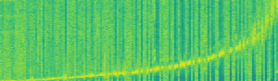
\includegraphics[interpolate=true,width=2.780000in,height=0.810000in]{figures/first_layer-img1.png}}%
\end{pgfscope}%
\begin{pgfscope}%
\pgfsetbuttcap%
\pgfsetroundjoin%
\definecolor{currentfill}{rgb}{0.000000,0.000000,0.000000}%
\pgfsetfillcolor{currentfill}%
\pgfsetlinewidth{0.803000pt}%
\definecolor{currentstroke}{rgb}{0.000000,0.000000,0.000000}%
\pgfsetstrokecolor{currentstroke}%
\pgfsetdash{}{0pt}%
\pgfsys@defobject{currentmarker}{\pgfqpoint{0.000000in}{-0.048611in}}{\pgfqpoint{0.000000in}{0.000000in}}{%
\pgfpathmoveto{\pgfqpoint{0.000000in}{0.000000in}}%
\pgfpathlineto{\pgfqpoint{0.000000in}{-0.048611in}}%
\pgfusepath{stroke,fill}%
}%
\begin{pgfscope}%
\pgfsys@transformshift{3.850554in}{2.909651in}%
\pgfsys@useobject{currentmarker}{}%
\end{pgfscope}%
\end{pgfscope}%
\begin{pgfscope}%
\definecolor{textcolor}{rgb}{0.000000,0.000000,0.000000}%
\pgfsetstrokecolor{textcolor}%
\pgfsetfillcolor{textcolor}%
\pgftext[x=3.850554in,y=2.812429in,,top]{\color{textcolor}\rmfamily\fontsize{10.000000}{12.000000}\selectfont \(\displaystyle {25}\)}%
\end{pgfscope}%
\begin{pgfscope}%
\pgfsetbuttcap%
\pgfsetroundjoin%
\definecolor{currentfill}{rgb}{0.000000,0.000000,0.000000}%
\pgfsetfillcolor{currentfill}%
\pgfsetlinewidth{0.803000pt}%
\definecolor{currentstroke}{rgb}{0.000000,0.000000,0.000000}%
\pgfsetstrokecolor{currentstroke}%
\pgfsetdash{}{0pt}%
\pgfsys@defobject{currentmarker}{\pgfqpoint{0.000000in}{-0.048611in}}{\pgfqpoint{0.000000in}{0.000000in}}{%
\pgfpathmoveto{\pgfqpoint{0.000000in}{0.000000in}}%
\pgfpathlineto{\pgfqpoint{0.000000in}{-0.048611in}}%
\pgfusepath{stroke,fill}%
}%
\begin{pgfscope}%
\pgfsys@transformshift{4.316675in}{2.909651in}%
\pgfsys@useobject{currentmarker}{}%
\end{pgfscope}%
\end{pgfscope}%
\begin{pgfscope}%
\definecolor{textcolor}{rgb}{0.000000,0.000000,0.000000}%
\pgfsetstrokecolor{textcolor}%
\pgfsetfillcolor{textcolor}%
\pgftext[x=4.316675in,y=2.812429in,,top]{\color{textcolor}\rmfamily\fontsize{10.000000}{12.000000}\selectfont \(\displaystyle {50}\)}%
\end{pgfscope}%
\begin{pgfscope}%
\pgfsetbuttcap%
\pgfsetroundjoin%
\definecolor{currentfill}{rgb}{0.000000,0.000000,0.000000}%
\pgfsetfillcolor{currentfill}%
\pgfsetlinewidth{0.803000pt}%
\definecolor{currentstroke}{rgb}{0.000000,0.000000,0.000000}%
\pgfsetstrokecolor{currentstroke}%
\pgfsetdash{}{0pt}%
\pgfsys@defobject{currentmarker}{\pgfqpoint{0.000000in}{-0.048611in}}{\pgfqpoint{0.000000in}{0.000000in}}{%
\pgfpathmoveto{\pgfqpoint{0.000000in}{0.000000in}}%
\pgfpathlineto{\pgfqpoint{0.000000in}{-0.048611in}}%
\pgfusepath{stroke,fill}%
}%
\begin{pgfscope}%
\pgfsys@transformshift{4.782795in}{2.909651in}%
\pgfsys@useobject{currentmarker}{}%
\end{pgfscope}%
\end{pgfscope}%
\begin{pgfscope}%
\definecolor{textcolor}{rgb}{0.000000,0.000000,0.000000}%
\pgfsetstrokecolor{textcolor}%
\pgfsetfillcolor{textcolor}%
\pgftext[x=4.782795in,y=2.812429in,,top]{\color{textcolor}\rmfamily\fontsize{10.000000}{12.000000}\selectfont \(\displaystyle {75}\)}%
\end{pgfscope}%
\begin{pgfscope}%
\pgfsetbuttcap%
\pgfsetroundjoin%
\definecolor{currentfill}{rgb}{0.000000,0.000000,0.000000}%
\pgfsetfillcolor{currentfill}%
\pgfsetlinewidth{0.803000pt}%
\definecolor{currentstroke}{rgb}{0.000000,0.000000,0.000000}%
\pgfsetstrokecolor{currentstroke}%
\pgfsetdash{}{0pt}%
\pgfsys@defobject{currentmarker}{\pgfqpoint{0.000000in}{-0.048611in}}{\pgfqpoint{0.000000in}{0.000000in}}{%
\pgfpathmoveto{\pgfqpoint{0.000000in}{0.000000in}}%
\pgfpathlineto{\pgfqpoint{0.000000in}{-0.048611in}}%
\pgfusepath{stroke,fill}%
}%
\begin{pgfscope}%
\pgfsys@transformshift{5.248916in}{2.909651in}%
\pgfsys@useobject{currentmarker}{}%
\end{pgfscope}%
\end{pgfscope}%
\begin{pgfscope}%
\definecolor{textcolor}{rgb}{0.000000,0.000000,0.000000}%
\pgfsetstrokecolor{textcolor}%
\pgfsetfillcolor{textcolor}%
\pgftext[x=5.248916in,y=2.812429in,,top]{\color{textcolor}\rmfamily\fontsize{10.000000}{12.000000}\selectfont \(\displaystyle {100}\)}%
\end{pgfscope}%
\begin{pgfscope}%
\pgfsetbuttcap%
\pgfsetroundjoin%
\definecolor{currentfill}{rgb}{0.000000,0.000000,0.000000}%
\pgfsetfillcolor{currentfill}%
\pgfsetlinewidth{0.803000pt}%
\definecolor{currentstroke}{rgb}{0.000000,0.000000,0.000000}%
\pgfsetstrokecolor{currentstroke}%
\pgfsetdash{}{0pt}%
\pgfsys@defobject{currentmarker}{\pgfqpoint{0.000000in}{-0.048611in}}{\pgfqpoint{0.000000in}{0.000000in}}{%
\pgfpathmoveto{\pgfqpoint{0.000000in}{0.000000in}}%
\pgfpathlineto{\pgfqpoint{0.000000in}{-0.048611in}}%
\pgfusepath{stroke,fill}%
}%
\begin{pgfscope}%
\pgfsys@transformshift{5.715036in}{2.909651in}%
\pgfsys@useobject{currentmarker}{}%
\end{pgfscope}%
\end{pgfscope}%
\begin{pgfscope}%
\definecolor{textcolor}{rgb}{0.000000,0.000000,0.000000}%
\pgfsetstrokecolor{textcolor}%
\pgfsetfillcolor{textcolor}%
\pgftext[x=5.715036in,y=2.812429in,,top]{\color{textcolor}\rmfamily\fontsize{10.000000}{12.000000}\selectfont \(\displaystyle {125}\)}%
\end{pgfscope}%
\begin{pgfscope}%
\pgfsetbuttcap%
\pgfsetroundjoin%
\definecolor{currentfill}{rgb}{0.000000,0.000000,0.000000}%
\pgfsetfillcolor{currentfill}%
\pgfsetlinewidth{0.803000pt}%
\definecolor{currentstroke}{rgb}{0.000000,0.000000,0.000000}%
\pgfsetstrokecolor{currentstroke}%
\pgfsetdash{}{0pt}%
\pgfsys@defobject{currentmarker}{\pgfqpoint{0.000000in}{-0.048611in}}{\pgfqpoint{0.000000in}{0.000000in}}{%
\pgfpathmoveto{\pgfqpoint{0.000000in}{0.000000in}}%
\pgfpathlineto{\pgfqpoint{0.000000in}{-0.048611in}}%
\pgfusepath{stroke,fill}%
}%
\begin{pgfscope}%
\pgfsys@transformshift{6.181157in}{2.909651in}%
\pgfsys@useobject{currentmarker}{}%
\end{pgfscope}%
\end{pgfscope}%
\begin{pgfscope}%
\definecolor{textcolor}{rgb}{0.000000,0.000000,0.000000}%
\pgfsetstrokecolor{textcolor}%
\pgfsetfillcolor{textcolor}%
\pgftext[x=6.181157in,y=2.812429in,,top]{\color{textcolor}\rmfamily\fontsize{10.000000}{12.000000}\selectfont \(\displaystyle {150}\)}%
\end{pgfscope}%
\begin{pgfscope}%
\pgfsetbuttcap%
\pgfsetroundjoin%
\definecolor{currentfill}{rgb}{0.000000,0.000000,0.000000}%
\pgfsetfillcolor{currentfill}%
\pgfsetlinewidth{0.803000pt}%
\definecolor{currentstroke}{rgb}{0.000000,0.000000,0.000000}%
\pgfsetstrokecolor{currentstroke}%
\pgfsetdash{}{0pt}%
\pgfsys@defobject{currentmarker}{\pgfqpoint{-0.048611in}{0.000000in}}{\pgfqpoint{-0.000000in}{0.000000in}}{%
\pgfpathmoveto{\pgfqpoint{-0.000000in}{0.000000in}}%
\pgfpathlineto{\pgfqpoint{-0.048611in}{0.000000in}}%
\pgfusepath{stroke,fill}%
}%
\begin{pgfscope}%
\pgfsys@transformshift{3.403079in}{2.909651in}%
\pgfsys@useobject{currentmarker}{}%
\end{pgfscope}%
\end{pgfscope}%
\begin{pgfscope}%
\definecolor{textcolor}{rgb}{0.000000,0.000000,0.000000}%
\pgfsetstrokecolor{textcolor}%
\pgfsetfillcolor{textcolor}%
\pgftext[x=3.236412in, y=2.861426in, left, base]{\color{textcolor}\rmfamily\fontsize{10.000000}{12.000000}\selectfont \(\displaystyle {0}\)}%
\end{pgfscope}%
\begin{pgfscope}%
\pgfsetbuttcap%
\pgfsetroundjoin%
\definecolor{currentfill}{rgb}{0.000000,0.000000,0.000000}%
\pgfsetfillcolor{currentfill}%
\pgfsetlinewidth{0.803000pt}%
\definecolor{currentstroke}{rgb}{0.000000,0.000000,0.000000}%
\pgfsetstrokecolor{currentstroke}%
\pgfsetdash{}{0pt}%
\pgfsys@defobject{currentmarker}{\pgfqpoint{-0.048611in}{0.000000in}}{\pgfqpoint{-0.000000in}{0.000000in}}{%
\pgfpathmoveto{\pgfqpoint{-0.000000in}{0.000000in}}%
\pgfpathlineto{\pgfqpoint{-0.048611in}{0.000000in}}%
\pgfusepath{stroke,fill}%
}%
\begin{pgfscope}%
\pgfsys@transformshift{3.403079in}{3.312218in}%
\pgfsys@useobject{currentmarker}{}%
\end{pgfscope}%
\end{pgfscope}%
\begin{pgfscope}%
\definecolor{textcolor}{rgb}{0.000000,0.000000,0.000000}%
\pgfsetstrokecolor{textcolor}%
\pgfsetfillcolor{textcolor}%
\pgftext[x=3.236412in, y=3.263993in, left, base]{\color{textcolor}\rmfamily\fontsize{10.000000}{12.000000}\selectfont \(\displaystyle {4}\)}%
\end{pgfscope}%
\begin{pgfscope}%
\pgfsetbuttcap%
\pgfsetroundjoin%
\definecolor{currentfill}{rgb}{0.000000,0.000000,0.000000}%
\pgfsetfillcolor{currentfill}%
\pgfsetlinewidth{0.803000pt}%
\definecolor{currentstroke}{rgb}{0.000000,0.000000,0.000000}%
\pgfsetstrokecolor{currentstroke}%
\pgfsetdash{}{0pt}%
\pgfsys@defobject{currentmarker}{\pgfqpoint{-0.048611in}{0.000000in}}{\pgfqpoint{-0.000000in}{0.000000in}}{%
\pgfpathmoveto{\pgfqpoint{-0.000000in}{0.000000in}}%
\pgfpathlineto{\pgfqpoint{-0.048611in}{0.000000in}}%
\pgfusepath{stroke,fill}%
}%
\begin{pgfscope}%
\pgfsys@transformshift{3.403079in}{3.714786in}%
\pgfsys@useobject{currentmarker}{}%
\end{pgfscope}%
\end{pgfscope}%
\begin{pgfscope}%
\definecolor{textcolor}{rgb}{0.000000,0.000000,0.000000}%
\pgfsetstrokecolor{textcolor}%
\pgfsetfillcolor{textcolor}%
\pgftext[x=3.236412in, y=3.666560in, left, base]{\color{textcolor}\rmfamily\fontsize{10.000000}{12.000000}\selectfont \(\displaystyle {8}\)}%
\end{pgfscope}%
\begin{pgfscope}%
\pgfsetrectcap%
\pgfsetmiterjoin%
\pgfsetlinewidth{0.803000pt}%
\definecolor{currentstroke}{rgb}{0.000000,0.000000,0.000000}%
\pgfsetstrokecolor{currentstroke}%
\pgfsetdash{}{0pt}%
\pgfpathmoveto{\pgfqpoint{3.403079in}{2.909651in}}%
\pgfpathlineto{\pgfqpoint{3.403079in}{3.714786in}}%
\pgfusepath{stroke}%
\end{pgfscope}%
\begin{pgfscope}%
\pgfsetrectcap%
\pgfsetmiterjoin%
\pgfsetlinewidth{0.803000pt}%
\definecolor{currentstroke}{rgb}{0.000000,0.000000,0.000000}%
\pgfsetstrokecolor{currentstroke}%
\pgfsetdash{}{0pt}%
\pgfpathmoveto{\pgfqpoint{6.181157in}{2.909651in}}%
\pgfpathlineto{\pgfqpoint{6.181157in}{3.714786in}}%
\pgfusepath{stroke}%
\end{pgfscope}%
\begin{pgfscope}%
\pgfsetrectcap%
\pgfsetmiterjoin%
\pgfsetlinewidth{0.803000pt}%
\definecolor{currentstroke}{rgb}{0.000000,0.000000,0.000000}%
\pgfsetstrokecolor{currentstroke}%
\pgfsetdash{}{0pt}%
\pgfpathmoveto{\pgfqpoint{3.403079in}{2.909651in}}%
\pgfpathlineto{\pgfqpoint{6.181157in}{2.909651in}}%
\pgfusepath{stroke}%
\end{pgfscope}%
\begin{pgfscope}%
\pgfsetrectcap%
\pgfsetmiterjoin%
\pgfsetlinewidth{0.803000pt}%
\definecolor{currentstroke}{rgb}{0.000000,0.000000,0.000000}%
\pgfsetstrokecolor{currentstroke}%
\pgfsetdash{}{0pt}%
\pgfpathmoveto{\pgfqpoint{3.403079in}{3.714786in}}%
\pgfpathlineto{\pgfqpoint{6.181157in}{3.714786in}}%
\pgfusepath{stroke}%
\end{pgfscope}%
\begin{pgfscope}%
\definecolor{textcolor}{rgb}{0.000000,0.000000,0.000000}%
\pgfsetstrokecolor{textcolor}%
\pgfsetfillcolor{textcolor}%
\pgftext[x=4.792118in,y=3.798119in,,base]{\color{textcolor}\rmfamily\fontsize{12.000000}{14.400000}\selectfont (b) SC}%
\end{pgfscope}%
\begin{pgfscope}%
\pgfsetbuttcap%
\pgfsetmiterjoin%
\definecolor{currentfill}{rgb}{1.000000,1.000000,1.000000}%
\pgfsetfillcolor{currentfill}%
\pgfsetlinewidth{0.000000pt}%
\definecolor{currentstroke}{rgb}{0.000000,0.000000,0.000000}%
\pgfsetstrokecolor{currentstroke}%
\pgfsetstrokeopacity{0.000000}%
\pgfsetdash{}{0pt}%
\pgfpathmoveto{\pgfqpoint{0.375000in}{1.661616in}}%
\pgfpathlineto{\pgfqpoint{3.153078in}{1.661616in}}%
\pgfpathlineto{\pgfqpoint{3.153078in}{2.466750in}}%
\pgfpathlineto{\pgfqpoint{0.375000in}{2.466750in}}%
\pgfpathlineto{\pgfqpoint{0.375000in}{1.661616in}}%
\pgfpathclose%
\pgfusepath{fill}%
\end{pgfscope}%
\begin{pgfscope}%
\pgfpathrectangle{\pgfqpoint{0.375000in}{1.661616in}}{\pgfqpoint{2.778078in}{0.805134in}}%
\pgfusepath{clip}%
\pgfsys@transformshift{0.375000in}{1.661616in}%
\pgftext[left,bottom]{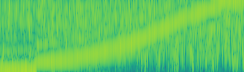
\includegraphics[interpolate=true,width=2.780000in,height=0.810000in]{figures/first_layer-img2.png}}%
\end{pgfscope}%
\begin{pgfscope}%
\pgfsetbuttcap%
\pgfsetroundjoin%
\definecolor{currentfill}{rgb}{0.000000,0.000000,0.000000}%
\pgfsetfillcolor{currentfill}%
\pgfsetlinewidth{0.803000pt}%
\definecolor{currentstroke}{rgb}{0.000000,0.000000,0.000000}%
\pgfsetstrokecolor{currentstroke}%
\pgfsetdash{}{0pt}%
\pgfsys@defobject{currentmarker}{\pgfqpoint{0.000000in}{-0.048611in}}{\pgfqpoint{0.000000in}{0.000000in}}{%
\pgfpathmoveto{\pgfqpoint{0.000000in}{0.000000in}}%
\pgfpathlineto{\pgfqpoint{0.000000in}{-0.048611in}}%
\pgfusepath{stroke,fill}%
}%
\begin{pgfscope}%
\pgfsys@transformshift{0.913219in}{1.661616in}%
\pgfsys@useobject{currentmarker}{}%
\end{pgfscope}%
\end{pgfscope}%
\begin{pgfscope}%
\definecolor{textcolor}{rgb}{0.000000,0.000000,0.000000}%
\pgfsetstrokecolor{textcolor}%
\pgfsetfillcolor{textcolor}%
\pgftext[x=0.913219in,y=1.564393in,,top]{\color{textcolor}\rmfamily\fontsize{10.000000}{12.000000}\selectfont \(\displaystyle {100}\)}%
\end{pgfscope}%
\begin{pgfscope}%
\pgfsetbuttcap%
\pgfsetroundjoin%
\definecolor{currentfill}{rgb}{0.000000,0.000000,0.000000}%
\pgfsetfillcolor{currentfill}%
\pgfsetlinewidth{0.803000pt}%
\definecolor{currentstroke}{rgb}{0.000000,0.000000,0.000000}%
\pgfsetstrokecolor{currentstroke}%
\pgfsetdash{}{0pt}%
\pgfsys@defobject{currentmarker}{\pgfqpoint{0.000000in}{-0.048611in}}{\pgfqpoint{0.000000in}{0.000000in}}{%
\pgfpathmoveto{\pgfqpoint{0.000000in}{0.000000in}}%
\pgfpathlineto{\pgfqpoint{0.000000in}{-0.048611in}}%
\pgfusepath{stroke,fill}%
}%
\begin{pgfscope}%
\pgfsys@transformshift{1.456874in}{1.661616in}%
\pgfsys@useobject{currentmarker}{}%
\end{pgfscope}%
\end{pgfscope}%
\begin{pgfscope}%
\definecolor{textcolor}{rgb}{0.000000,0.000000,0.000000}%
\pgfsetstrokecolor{textcolor}%
\pgfsetfillcolor{textcolor}%
\pgftext[x=1.456874in,y=1.564393in,,top]{\color{textcolor}\rmfamily\fontsize{10.000000}{12.000000}\selectfont \(\displaystyle {200}\)}%
\end{pgfscope}%
\begin{pgfscope}%
\pgfsetbuttcap%
\pgfsetroundjoin%
\definecolor{currentfill}{rgb}{0.000000,0.000000,0.000000}%
\pgfsetfillcolor{currentfill}%
\pgfsetlinewidth{0.803000pt}%
\definecolor{currentstroke}{rgb}{0.000000,0.000000,0.000000}%
\pgfsetstrokecolor{currentstroke}%
\pgfsetdash{}{0pt}%
\pgfsys@defobject{currentmarker}{\pgfqpoint{0.000000in}{-0.048611in}}{\pgfqpoint{0.000000in}{0.000000in}}{%
\pgfpathmoveto{\pgfqpoint{0.000000in}{0.000000in}}%
\pgfpathlineto{\pgfqpoint{0.000000in}{-0.048611in}}%
\pgfusepath{stroke,fill}%
}%
\begin{pgfscope}%
\pgfsys@transformshift{2.000529in}{1.661616in}%
\pgfsys@useobject{currentmarker}{}%
\end{pgfscope}%
\end{pgfscope}%
\begin{pgfscope}%
\definecolor{textcolor}{rgb}{0.000000,0.000000,0.000000}%
\pgfsetstrokecolor{textcolor}%
\pgfsetfillcolor{textcolor}%
\pgftext[x=2.000529in,y=1.564393in,,top]{\color{textcolor}\rmfamily\fontsize{10.000000}{12.000000}\selectfont \(\displaystyle {300}\)}%
\end{pgfscope}%
\begin{pgfscope}%
\pgfsetbuttcap%
\pgfsetroundjoin%
\definecolor{currentfill}{rgb}{0.000000,0.000000,0.000000}%
\pgfsetfillcolor{currentfill}%
\pgfsetlinewidth{0.803000pt}%
\definecolor{currentstroke}{rgb}{0.000000,0.000000,0.000000}%
\pgfsetstrokecolor{currentstroke}%
\pgfsetdash{}{0pt}%
\pgfsys@defobject{currentmarker}{\pgfqpoint{0.000000in}{-0.048611in}}{\pgfqpoint{0.000000in}{0.000000in}}{%
\pgfpathmoveto{\pgfqpoint{0.000000in}{0.000000in}}%
\pgfpathlineto{\pgfqpoint{0.000000in}{-0.048611in}}%
\pgfusepath{stroke,fill}%
}%
\begin{pgfscope}%
\pgfsys@transformshift{2.544184in}{1.661616in}%
\pgfsys@useobject{currentmarker}{}%
\end{pgfscope}%
\end{pgfscope}%
\begin{pgfscope}%
\definecolor{textcolor}{rgb}{0.000000,0.000000,0.000000}%
\pgfsetstrokecolor{textcolor}%
\pgfsetfillcolor{textcolor}%
\pgftext[x=2.544184in,y=1.564393in,,top]{\color{textcolor}\rmfamily\fontsize{10.000000}{12.000000}\selectfont \(\displaystyle {400}\)}%
\end{pgfscope}%
\begin{pgfscope}%
\pgfsetbuttcap%
\pgfsetroundjoin%
\definecolor{currentfill}{rgb}{0.000000,0.000000,0.000000}%
\pgfsetfillcolor{currentfill}%
\pgfsetlinewidth{0.803000pt}%
\definecolor{currentstroke}{rgb}{0.000000,0.000000,0.000000}%
\pgfsetstrokecolor{currentstroke}%
\pgfsetdash{}{0pt}%
\pgfsys@defobject{currentmarker}{\pgfqpoint{0.000000in}{-0.048611in}}{\pgfqpoint{0.000000in}{0.000000in}}{%
\pgfpathmoveto{\pgfqpoint{0.000000in}{0.000000in}}%
\pgfpathlineto{\pgfqpoint{0.000000in}{-0.048611in}}%
\pgfusepath{stroke,fill}%
}%
\begin{pgfscope}%
\pgfsys@transformshift{3.087840in}{1.661616in}%
\pgfsys@useobject{currentmarker}{}%
\end{pgfscope}%
\end{pgfscope}%
\begin{pgfscope}%
\definecolor{textcolor}{rgb}{0.000000,0.000000,0.000000}%
\pgfsetstrokecolor{textcolor}%
\pgfsetfillcolor{textcolor}%
\pgftext[x=3.087840in,y=1.564393in,,top]{\color{textcolor}\rmfamily\fontsize{10.000000}{12.000000}\selectfont \(\displaystyle {500}\)}%
\end{pgfscope}%
\begin{pgfscope}%
\pgfsetbuttcap%
\pgfsetroundjoin%
\definecolor{currentfill}{rgb}{0.000000,0.000000,0.000000}%
\pgfsetfillcolor{currentfill}%
\pgfsetlinewidth{0.803000pt}%
\definecolor{currentstroke}{rgb}{0.000000,0.000000,0.000000}%
\pgfsetstrokecolor{currentstroke}%
\pgfsetdash{}{0pt}%
\pgfsys@defobject{currentmarker}{\pgfqpoint{-0.048611in}{0.000000in}}{\pgfqpoint{-0.000000in}{0.000000in}}{%
\pgfpathmoveto{\pgfqpoint{-0.000000in}{0.000000in}}%
\pgfpathlineto{\pgfqpoint{-0.048611in}{0.000000in}}%
\pgfusepath{stroke,fill}%
}%
\begin{pgfscope}%
\pgfsys@transformshift{0.375000in}{1.661616in}%
\pgfsys@useobject{currentmarker}{}%
\end{pgfscope}%
\end{pgfscope}%
\begin{pgfscope}%
\definecolor{textcolor}{rgb}{0.000000,0.000000,0.000000}%
\pgfsetstrokecolor{textcolor}%
\pgfsetfillcolor{textcolor}%
\pgftext[x=0.208333in, y=1.613390in, left, base]{\color{textcolor}\rmfamily\fontsize{10.000000}{12.000000}\selectfont \(\displaystyle {0}\)}%
\end{pgfscope}%
\begin{pgfscope}%
\pgfsetbuttcap%
\pgfsetroundjoin%
\definecolor{currentfill}{rgb}{0.000000,0.000000,0.000000}%
\pgfsetfillcolor{currentfill}%
\pgfsetlinewidth{0.803000pt}%
\definecolor{currentstroke}{rgb}{0.000000,0.000000,0.000000}%
\pgfsetstrokecolor{currentstroke}%
\pgfsetdash{}{0pt}%
\pgfsys@defobject{currentmarker}{\pgfqpoint{-0.048611in}{0.000000in}}{\pgfqpoint{-0.000000in}{0.000000in}}{%
\pgfpathmoveto{\pgfqpoint{-0.000000in}{0.000000in}}%
\pgfpathlineto{\pgfqpoint{-0.048611in}{0.000000in}}%
\pgfusepath{stroke,fill}%
}%
\begin{pgfscope}%
\pgfsys@transformshift{0.375000in}{2.064183in}%
\pgfsys@useobject{currentmarker}{}%
\end{pgfscope}%
\end{pgfscope}%
\begin{pgfscope}%
\definecolor{textcolor}{rgb}{0.000000,0.000000,0.000000}%
\pgfsetstrokecolor{textcolor}%
\pgfsetfillcolor{textcolor}%
\pgftext[x=0.208333in, y=2.015958in, left, base]{\color{textcolor}\rmfamily\fontsize{10.000000}{12.000000}\selectfont \(\displaystyle {4}\)}%
\end{pgfscope}%
\begin{pgfscope}%
\pgfsetbuttcap%
\pgfsetroundjoin%
\definecolor{currentfill}{rgb}{0.000000,0.000000,0.000000}%
\pgfsetfillcolor{currentfill}%
\pgfsetlinewidth{0.803000pt}%
\definecolor{currentstroke}{rgb}{0.000000,0.000000,0.000000}%
\pgfsetstrokecolor{currentstroke}%
\pgfsetdash{}{0pt}%
\pgfsys@defobject{currentmarker}{\pgfqpoint{-0.048611in}{0.000000in}}{\pgfqpoint{-0.000000in}{0.000000in}}{%
\pgfpathmoveto{\pgfqpoint{-0.000000in}{0.000000in}}%
\pgfpathlineto{\pgfqpoint{-0.048611in}{0.000000in}}%
\pgfusepath{stroke,fill}%
}%
\begin{pgfscope}%
\pgfsys@transformshift{0.375000in}{2.466750in}%
\pgfsys@useobject{currentmarker}{}%
\end{pgfscope}%
\end{pgfscope}%
\begin{pgfscope}%
\definecolor{textcolor}{rgb}{0.000000,0.000000,0.000000}%
\pgfsetstrokecolor{textcolor}%
\pgfsetfillcolor{textcolor}%
\pgftext[x=0.208333in, y=2.418525in, left, base]{\color{textcolor}\rmfamily\fontsize{10.000000}{12.000000}\selectfont \(\displaystyle {8}\)}%
\end{pgfscope}%
\begin{pgfscope}%
\definecolor{textcolor}{rgb}{0.000000,0.000000,0.000000}%
\pgfsetstrokecolor{textcolor}%
\pgfsetfillcolor{textcolor}%
\pgftext[x=0.152778in,y=2.064183in,,bottom,rotate=90.000000]{\color{textcolor}\rmfamily\fontsize{10.000000}{12.000000}\selectfont Frequency [\si{\kilo\hertz}]}%
\end{pgfscope}%
\begin{pgfscope}%
\pgfsetrectcap%
\pgfsetmiterjoin%
\pgfsetlinewidth{0.803000pt}%
\definecolor{currentstroke}{rgb}{0.000000,0.000000,0.000000}%
\pgfsetstrokecolor{currentstroke}%
\pgfsetdash{}{0pt}%
\pgfpathmoveto{\pgfqpoint{0.375000in}{1.661616in}}%
\pgfpathlineto{\pgfqpoint{0.375000in}{2.466750in}}%
\pgfusepath{stroke}%
\end{pgfscope}%
\begin{pgfscope}%
\pgfsetrectcap%
\pgfsetmiterjoin%
\pgfsetlinewidth{0.803000pt}%
\definecolor{currentstroke}{rgb}{0.000000,0.000000,0.000000}%
\pgfsetstrokecolor{currentstroke}%
\pgfsetdash{}{0pt}%
\pgfpathmoveto{\pgfqpoint{3.153078in}{1.661616in}}%
\pgfpathlineto{\pgfqpoint{3.153078in}{2.466750in}}%
\pgfusepath{stroke}%
\end{pgfscope}%
\begin{pgfscope}%
\pgfsetrectcap%
\pgfsetmiterjoin%
\pgfsetlinewidth{0.803000pt}%
\definecolor{currentstroke}{rgb}{0.000000,0.000000,0.000000}%
\pgfsetstrokecolor{currentstroke}%
\pgfsetdash{}{0pt}%
\pgfpathmoveto{\pgfqpoint{0.375000in}{1.661616in}}%
\pgfpathlineto{\pgfqpoint{3.153078in}{1.661616in}}%
\pgfusepath{stroke}%
\end{pgfscope}%
\begin{pgfscope}%
\pgfsetrectcap%
\pgfsetmiterjoin%
\pgfsetlinewidth{0.803000pt}%
\definecolor{currentstroke}{rgb}{0.000000,0.000000,0.000000}%
\pgfsetstrokecolor{currentstroke}%
\pgfsetdash{}{0pt}%
\pgfpathmoveto{\pgfqpoint{0.375000in}{2.466750in}}%
\pgfpathlineto{\pgfqpoint{3.153078in}{2.466750in}}%
\pgfusepath{stroke}%
\end{pgfscope}%
\begin{pgfscope}%
\definecolor{textcolor}{rgb}{0.000000,0.000000,0.000000}%
\pgfsetstrokecolor{textcolor}%
\pgfsetfillcolor{textcolor}%
\pgftext[x=1.764039in,y=2.550083in,,base]{\color{textcolor}\rmfamily\fontsize{12.000000}{14.400000}\selectfont (c) wav2vec 2.0 FE}%
\end{pgfscope}%
\begin{pgfscope}%
\pgfsetbuttcap%
\pgfsetmiterjoin%
\definecolor{currentfill}{rgb}{1.000000,1.000000,1.000000}%
\pgfsetfillcolor{currentfill}%
\pgfsetlinewidth{0.000000pt}%
\definecolor{currentstroke}{rgb}{0.000000,0.000000,0.000000}%
\pgfsetstrokecolor{currentstroke}%
\pgfsetstrokeopacity{0.000000}%
\pgfsetdash{}{0pt}%
\pgfpathmoveto{\pgfqpoint{3.403079in}{1.661616in}}%
\pgfpathlineto{\pgfqpoint{6.181157in}{1.661616in}}%
\pgfpathlineto{\pgfqpoint{6.181157in}{2.466750in}}%
\pgfpathlineto{\pgfqpoint{3.403079in}{2.466750in}}%
\pgfpathlineto{\pgfqpoint{3.403079in}{1.661616in}}%
\pgfpathclose%
\pgfusepath{fill}%
\end{pgfscope}%
\begin{pgfscope}%
\pgfpathrectangle{\pgfqpoint{3.403079in}{1.661616in}}{\pgfqpoint{2.778078in}{0.805134in}}%
\pgfusepath{clip}%
\pgfsys@transformshift{3.403079in}{1.661616in}%
\pgftext[left,bottom]{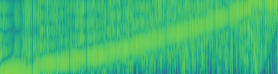
\includegraphics[interpolate=true,width=2.780000in,height=0.810000in]{figures/first_layer-img3.png}}%
\end{pgfscope}%
\begin{pgfscope}%
\pgfsetbuttcap%
\pgfsetroundjoin%
\definecolor{currentfill}{rgb}{0.000000,0.000000,0.000000}%
\pgfsetfillcolor{currentfill}%
\pgfsetlinewidth{0.803000pt}%
\definecolor{currentstroke}{rgb}{0.000000,0.000000,0.000000}%
\pgfsetstrokecolor{currentstroke}%
\pgfsetdash{}{0pt}%
\pgfsys@defobject{currentmarker}{\pgfqpoint{0.000000in}{-0.048611in}}{\pgfqpoint{0.000000in}{0.000000in}}{%
\pgfpathmoveto{\pgfqpoint{0.000000in}{0.000000in}}%
\pgfpathlineto{\pgfqpoint{0.000000in}{-0.048611in}}%
\pgfusepath{stroke,fill}%
}%
\begin{pgfscope}%
\pgfsys@transformshift{3.941297in}{1.661616in}%
\pgfsys@useobject{currentmarker}{}%
\end{pgfscope}%
\end{pgfscope}%
\begin{pgfscope}%
\definecolor{textcolor}{rgb}{0.000000,0.000000,0.000000}%
\pgfsetstrokecolor{textcolor}%
\pgfsetfillcolor{textcolor}%
\pgftext[x=3.941297in,y=1.564393in,,top]{\color{textcolor}\rmfamily\fontsize{10.000000}{12.000000}\selectfont \(\displaystyle {100}\)}%
\end{pgfscope}%
\begin{pgfscope}%
\pgfsetbuttcap%
\pgfsetroundjoin%
\definecolor{currentfill}{rgb}{0.000000,0.000000,0.000000}%
\pgfsetfillcolor{currentfill}%
\pgfsetlinewidth{0.803000pt}%
\definecolor{currentstroke}{rgb}{0.000000,0.000000,0.000000}%
\pgfsetstrokecolor{currentstroke}%
\pgfsetdash{}{0pt}%
\pgfsys@defobject{currentmarker}{\pgfqpoint{0.000000in}{-0.048611in}}{\pgfqpoint{0.000000in}{0.000000in}}{%
\pgfpathmoveto{\pgfqpoint{0.000000in}{0.000000in}}%
\pgfpathlineto{\pgfqpoint{0.000000in}{-0.048611in}}%
\pgfusepath{stroke,fill}%
}%
\begin{pgfscope}%
\pgfsys@transformshift{4.484953in}{1.661616in}%
\pgfsys@useobject{currentmarker}{}%
\end{pgfscope}%
\end{pgfscope}%
\begin{pgfscope}%
\definecolor{textcolor}{rgb}{0.000000,0.000000,0.000000}%
\pgfsetstrokecolor{textcolor}%
\pgfsetfillcolor{textcolor}%
\pgftext[x=4.484953in,y=1.564393in,,top]{\color{textcolor}\rmfamily\fontsize{10.000000}{12.000000}\selectfont \(\displaystyle {200}\)}%
\end{pgfscope}%
\begin{pgfscope}%
\pgfsetbuttcap%
\pgfsetroundjoin%
\definecolor{currentfill}{rgb}{0.000000,0.000000,0.000000}%
\pgfsetfillcolor{currentfill}%
\pgfsetlinewidth{0.803000pt}%
\definecolor{currentstroke}{rgb}{0.000000,0.000000,0.000000}%
\pgfsetstrokecolor{currentstroke}%
\pgfsetdash{}{0pt}%
\pgfsys@defobject{currentmarker}{\pgfqpoint{0.000000in}{-0.048611in}}{\pgfqpoint{0.000000in}{0.000000in}}{%
\pgfpathmoveto{\pgfqpoint{0.000000in}{0.000000in}}%
\pgfpathlineto{\pgfqpoint{0.000000in}{-0.048611in}}%
\pgfusepath{stroke,fill}%
}%
\begin{pgfscope}%
\pgfsys@transformshift{5.028608in}{1.661616in}%
\pgfsys@useobject{currentmarker}{}%
\end{pgfscope}%
\end{pgfscope}%
\begin{pgfscope}%
\definecolor{textcolor}{rgb}{0.000000,0.000000,0.000000}%
\pgfsetstrokecolor{textcolor}%
\pgfsetfillcolor{textcolor}%
\pgftext[x=5.028608in,y=1.564393in,,top]{\color{textcolor}\rmfamily\fontsize{10.000000}{12.000000}\selectfont \(\displaystyle {300}\)}%
\end{pgfscope}%
\begin{pgfscope}%
\pgfsetbuttcap%
\pgfsetroundjoin%
\definecolor{currentfill}{rgb}{0.000000,0.000000,0.000000}%
\pgfsetfillcolor{currentfill}%
\pgfsetlinewidth{0.803000pt}%
\definecolor{currentstroke}{rgb}{0.000000,0.000000,0.000000}%
\pgfsetstrokecolor{currentstroke}%
\pgfsetdash{}{0pt}%
\pgfsys@defobject{currentmarker}{\pgfqpoint{0.000000in}{-0.048611in}}{\pgfqpoint{0.000000in}{0.000000in}}{%
\pgfpathmoveto{\pgfqpoint{0.000000in}{0.000000in}}%
\pgfpathlineto{\pgfqpoint{0.000000in}{-0.048611in}}%
\pgfusepath{stroke,fill}%
}%
\begin{pgfscope}%
\pgfsys@transformshift{5.572263in}{1.661616in}%
\pgfsys@useobject{currentmarker}{}%
\end{pgfscope}%
\end{pgfscope}%
\begin{pgfscope}%
\definecolor{textcolor}{rgb}{0.000000,0.000000,0.000000}%
\pgfsetstrokecolor{textcolor}%
\pgfsetfillcolor{textcolor}%
\pgftext[x=5.572263in,y=1.564393in,,top]{\color{textcolor}\rmfamily\fontsize{10.000000}{12.000000}\selectfont \(\displaystyle {400}\)}%
\end{pgfscope}%
\begin{pgfscope}%
\pgfsetbuttcap%
\pgfsetroundjoin%
\definecolor{currentfill}{rgb}{0.000000,0.000000,0.000000}%
\pgfsetfillcolor{currentfill}%
\pgfsetlinewidth{0.803000pt}%
\definecolor{currentstroke}{rgb}{0.000000,0.000000,0.000000}%
\pgfsetstrokecolor{currentstroke}%
\pgfsetdash{}{0pt}%
\pgfsys@defobject{currentmarker}{\pgfqpoint{0.000000in}{-0.048611in}}{\pgfqpoint{0.000000in}{0.000000in}}{%
\pgfpathmoveto{\pgfqpoint{0.000000in}{0.000000in}}%
\pgfpathlineto{\pgfqpoint{0.000000in}{-0.048611in}}%
\pgfusepath{stroke,fill}%
}%
\begin{pgfscope}%
\pgfsys@transformshift{6.115918in}{1.661616in}%
\pgfsys@useobject{currentmarker}{}%
\end{pgfscope}%
\end{pgfscope}%
\begin{pgfscope}%
\definecolor{textcolor}{rgb}{0.000000,0.000000,0.000000}%
\pgfsetstrokecolor{textcolor}%
\pgfsetfillcolor{textcolor}%
\pgftext[x=6.115918in,y=1.564393in,,top]{\color{textcolor}\rmfamily\fontsize{10.000000}{12.000000}\selectfont \(\displaystyle {500}\)}%
\end{pgfscope}%
\begin{pgfscope}%
\pgfsetbuttcap%
\pgfsetroundjoin%
\definecolor{currentfill}{rgb}{0.000000,0.000000,0.000000}%
\pgfsetfillcolor{currentfill}%
\pgfsetlinewidth{0.803000pt}%
\definecolor{currentstroke}{rgb}{0.000000,0.000000,0.000000}%
\pgfsetstrokecolor{currentstroke}%
\pgfsetdash{}{0pt}%
\pgfsys@defobject{currentmarker}{\pgfqpoint{-0.048611in}{0.000000in}}{\pgfqpoint{-0.000000in}{0.000000in}}{%
\pgfpathmoveto{\pgfqpoint{-0.000000in}{0.000000in}}%
\pgfpathlineto{\pgfqpoint{-0.048611in}{0.000000in}}%
\pgfusepath{stroke,fill}%
}%
\begin{pgfscope}%
\pgfsys@transformshift{3.403079in}{1.661616in}%
\pgfsys@useobject{currentmarker}{}%
\end{pgfscope}%
\end{pgfscope}%
\begin{pgfscope}%
\definecolor{textcolor}{rgb}{0.000000,0.000000,0.000000}%
\pgfsetstrokecolor{textcolor}%
\pgfsetfillcolor{textcolor}%
\pgftext[x=3.236412in, y=1.613390in, left, base]{\color{textcolor}\rmfamily\fontsize{10.000000}{12.000000}\selectfont \(\displaystyle {0}\)}%
\end{pgfscope}%
\begin{pgfscope}%
\pgfsetbuttcap%
\pgfsetroundjoin%
\definecolor{currentfill}{rgb}{0.000000,0.000000,0.000000}%
\pgfsetfillcolor{currentfill}%
\pgfsetlinewidth{0.803000pt}%
\definecolor{currentstroke}{rgb}{0.000000,0.000000,0.000000}%
\pgfsetstrokecolor{currentstroke}%
\pgfsetdash{}{0pt}%
\pgfsys@defobject{currentmarker}{\pgfqpoint{-0.048611in}{0.000000in}}{\pgfqpoint{-0.000000in}{0.000000in}}{%
\pgfpathmoveto{\pgfqpoint{-0.000000in}{0.000000in}}%
\pgfpathlineto{\pgfqpoint{-0.048611in}{0.000000in}}%
\pgfusepath{stroke,fill}%
}%
\begin{pgfscope}%
\pgfsys@transformshift{3.403079in}{2.064183in}%
\pgfsys@useobject{currentmarker}{}%
\end{pgfscope}%
\end{pgfscope}%
\begin{pgfscope}%
\definecolor{textcolor}{rgb}{0.000000,0.000000,0.000000}%
\pgfsetstrokecolor{textcolor}%
\pgfsetfillcolor{textcolor}%
\pgftext[x=3.236412in, y=2.015958in, left, base]{\color{textcolor}\rmfamily\fontsize{10.000000}{12.000000}\selectfont \(\displaystyle {4}\)}%
\end{pgfscope}%
\begin{pgfscope}%
\pgfsetbuttcap%
\pgfsetroundjoin%
\definecolor{currentfill}{rgb}{0.000000,0.000000,0.000000}%
\pgfsetfillcolor{currentfill}%
\pgfsetlinewidth{0.803000pt}%
\definecolor{currentstroke}{rgb}{0.000000,0.000000,0.000000}%
\pgfsetstrokecolor{currentstroke}%
\pgfsetdash{}{0pt}%
\pgfsys@defobject{currentmarker}{\pgfqpoint{-0.048611in}{0.000000in}}{\pgfqpoint{-0.000000in}{0.000000in}}{%
\pgfpathmoveto{\pgfqpoint{-0.000000in}{0.000000in}}%
\pgfpathlineto{\pgfqpoint{-0.048611in}{0.000000in}}%
\pgfusepath{stroke,fill}%
}%
\begin{pgfscope}%
\pgfsys@transformshift{3.403079in}{2.466750in}%
\pgfsys@useobject{currentmarker}{}%
\end{pgfscope}%
\end{pgfscope}%
\begin{pgfscope}%
\definecolor{textcolor}{rgb}{0.000000,0.000000,0.000000}%
\pgfsetstrokecolor{textcolor}%
\pgfsetfillcolor{textcolor}%
\pgftext[x=3.236412in, y=2.418525in, left, base]{\color{textcolor}\rmfamily\fontsize{10.000000}{12.000000}\selectfont \(\displaystyle {8}\)}%
\end{pgfscope}%
\begin{pgfscope}%
\pgfsetrectcap%
\pgfsetmiterjoin%
\pgfsetlinewidth{0.803000pt}%
\definecolor{currentstroke}{rgb}{0.000000,0.000000,0.000000}%
\pgfsetstrokecolor{currentstroke}%
\pgfsetdash{}{0pt}%
\pgfpathmoveto{\pgfqpoint{3.403079in}{1.661616in}}%
\pgfpathlineto{\pgfqpoint{3.403079in}{2.466750in}}%
\pgfusepath{stroke}%
\end{pgfscope}%
\begin{pgfscope}%
\pgfsetrectcap%
\pgfsetmiterjoin%
\pgfsetlinewidth{0.803000pt}%
\definecolor{currentstroke}{rgb}{0.000000,0.000000,0.000000}%
\pgfsetstrokecolor{currentstroke}%
\pgfsetdash{}{0pt}%
\pgfpathmoveto{\pgfqpoint{6.181157in}{1.661616in}}%
\pgfpathlineto{\pgfqpoint{6.181157in}{2.466750in}}%
\pgfusepath{stroke}%
\end{pgfscope}%
\begin{pgfscope}%
\pgfsetrectcap%
\pgfsetmiterjoin%
\pgfsetlinewidth{0.803000pt}%
\definecolor{currentstroke}{rgb}{0.000000,0.000000,0.000000}%
\pgfsetstrokecolor{currentstroke}%
\pgfsetdash{}{0pt}%
\pgfpathmoveto{\pgfqpoint{3.403079in}{1.661616in}}%
\pgfpathlineto{\pgfqpoint{6.181157in}{1.661616in}}%
\pgfusepath{stroke}%
\end{pgfscope}%
\begin{pgfscope}%
\pgfsetrectcap%
\pgfsetmiterjoin%
\pgfsetlinewidth{0.803000pt}%
\definecolor{currentstroke}{rgb}{0.000000,0.000000,0.000000}%
\pgfsetstrokecolor{currentstroke}%
\pgfsetdash{}{0pt}%
\pgfpathmoveto{\pgfqpoint{3.403079in}{2.466750in}}%
\pgfpathlineto{\pgfqpoint{6.181157in}{2.466750in}}%
\pgfusepath{stroke}%
\end{pgfscope}%
\begin{pgfscope}%
\definecolor{textcolor}{rgb}{0.000000,0.000000,0.000000}%
\pgfsetstrokecolor{textcolor}%
\pgfsetfillcolor{textcolor}%
\pgftext[x=4.792118in,y=2.550083in,,base]{\color{textcolor}\rmfamily\fontsize{12.000000}{14.400000}\selectfont (d) wav2vec 2.0 FE (pre-training)}%
\end{pgfscope}%
\begin{pgfscope}%
\pgfsetbuttcap%
\pgfsetmiterjoin%
\definecolor{currentfill}{rgb}{1.000000,1.000000,1.000000}%
\pgfsetfillcolor{currentfill}%
\pgfsetlinewidth{0.000000pt}%
\definecolor{currentstroke}{rgb}{0.000000,0.000000,0.000000}%
\pgfsetstrokecolor{currentstroke}%
\pgfsetstrokeopacity{0.000000}%
\pgfsetdash{}{0pt}%
\pgfpathmoveto{\pgfqpoint{0.375000in}{0.413580in}}%
\pgfpathlineto{\pgfqpoint{3.153078in}{0.413580in}}%
\pgfpathlineto{\pgfqpoint{3.153078in}{1.218714in}}%
\pgfpathlineto{\pgfqpoint{0.375000in}{1.218714in}}%
\pgfpathlineto{\pgfqpoint{0.375000in}{0.413580in}}%
\pgfpathclose%
\pgfusepath{fill}%
\end{pgfscope}%
\begin{pgfscope}%
\pgfpathrectangle{\pgfqpoint{0.375000in}{0.413580in}}{\pgfqpoint{2.778078in}{0.805134in}}%
\pgfusepath{clip}%
\pgfsys@transformshift{0.375000in}{0.413580in}%
\pgftext[left,bottom]{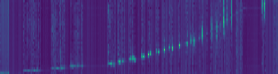
\includegraphics[interpolate=true,width=2.780000in,height=0.810000in]{figures/first_layer-img4.png}}%
\end{pgfscope}%
\begin{pgfscope}%
\pgfsetbuttcap%
\pgfsetroundjoin%
\definecolor{currentfill}{rgb}{0.000000,0.000000,0.000000}%
\pgfsetfillcolor{currentfill}%
\pgfsetlinewidth{0.803000pt}%
\definecolor{currentstroke}{rgb}{0.000000,0.000000,0.000000}%
\pgfsetstrokecolor{currentstroke}%
\pgfsetdash{}{0pt}%
\pgfsys@defobject{currentmarker}{\pgfqpoint{0.000000in}{-0.048611in}}{\pgfqpoint{0.000000in}{0.000000in}}{%
\pgfpathmoveto{\pgfqpoint{0.000000in}{0.000000in}}%
\pgfpathlineto{\pgfqpoint{0.000000in}{-0.048611in}}%
\pgfusepath{stroke,fill}%
}%
\begin{pgfscope}%
\pgfsys@transformshift{1.113101in}{0.413580in}%
\pgfsys@useobject{currentmarker}{}%
\end{pgfscope}%
\end{pgfscope}%
\begin{pgfscope}%
\definecolor{textcolor}{rgb}{0.000000,0.000000,0.000000}%
\pgfsetstrokecolor{textcolor}%
\pgfsetfillcolor{textcolor}%
\pgftext[x=1.113101in,y=0.316358in,,top]{\color{textcolor}\rmfamily\fontsize{10.000000}{12.000000}\selectfont \(\displaystyle {200}\)}%
\end{pgfscope}%
\begin{pgfscope}%
\pgfsetbuttcap%
\pgfsetroundjoin%
\definecolor{currentfill}{rgb}{0.000000,0.000000,0.000000}%
\pgfsetfillcolor{currentfill}%
\pgfsetlinewidth{0.803000pt}%
\definecolor{currentstroke}{rgb}{0.000000,0.000000,0.000000}%
\pgfsetstrokecolor{currentstroke}%
\pgfsetdash{}{0pt}%
\pgfsys@defobject{currentmarker}{\pgfqpoint{0.000000in}{-0.048611in}}{\pgfqpoint{0.000000in}{0.000000in}}{%
\pgfpathmoveto{\pgfqpoint{0.000000in}{0.000000in}}%
\pgfpathlineto{\pgfqpoint{0.000000in}{-0.048611in}}%
\pgfusepath{stroke,fill}%
}%
\begin{pgfscope}%
\pgfsys@transformshift{1.854911in}{0.413580in}%
\pgfsys@useobject{currentmarker}{}%
\end{pgfscope}%
\end{pgfscope}%
\begin{pgfscope}%
\definecolor{textcolor}{rgb}{0.000000,0.000000,0.000000}%
\pgfsetstrokecolor{textcolor}%
\pgfsetfillcolor{textcolor}%
\pgftext[x=1.854911in,y=0.316358in,,top]{\color{textcolor}\rmfamily\fontsize{10.000000}{12.000000}\selectfont \(\displaystyle {400}\)}%
\end{pgfscope}%
\begin{pgfscope}%
\pgfsetbuttcap%
\pgfsetroundjoin%
\definecolor{currentfill}{rgb}{0.000000,0.000000,0.000000}%
\pgfsetfillcolor{currentfill}%
\pgfsetlinewidth{0.803000pt}%
\definecolor{currentstroke}{rgb}{0.000000,0.000000,0.000000}%
\pgfsetstrokecolor{currentstroke}%
\pgfsetdash{}{0pt}%
\pgfsys@defobject{currentmarker}{\pgfqpoint{0.000000in}{-0.048611in}}{\pgfqpoint{0.000000in}{0.000000in}}{%
\pgfpathmoveto{\pgfqpoint{0.000000in}{0.000000in}}%
\pgfpathlineto{\pgfqpoint{0.000000in}{-0.048611in}}%
\pgfusepath{stroke,fill}%
}%
\begin{pgfscope}%
\pgfsys@transformshift{2.596721in}{0.413580in}%
\pgfsys@useobject{currentmarker}{}%
\end{pgfscope}%
\end{pgfscope}%
\begin{pgfscope}%
\definecolor{textcolor}{rgb}{0.000000,0.000000,0.000000}%
\pgfsetstrokecolor{textcolor}%
\pgfsetfillcolor{textcolor}%
\pgftext[x=2.596721in,y=0.316358in,,top]{\color{textcolor}\rmfamily\fontsize{10.000000}{12.000000}\selectfont \(\displaystyle {600}\)}%
\end{pgfscope}%
\begin{pgfscope}%
\definecolor{textcolor}{rgb}{0.000000,0.000000,0.000000}%
\pgfsetstrokecolor{textcolor}%
\pgfsetfillcolor{textcolor}%
\pgftext[x=1.764039in,y=0.137346in,,top]{\color{textcolor}\rmfamily\fontsize{10.000000}{12.000000}\selectfont Filter index}%
\end{pgfscope}%
\begin{pgfscope}%
\pgfsetbuttcap%
\pgfsetroundjoin%
\definecolor{currentfill}{rgb}{0.000000,0.000000,0.000000}%
\pgfsetfillcolor{currentfill}%
\pgfsetlinewidth{0.803000pt}%
\definecolor{currentstroke}{rgb}{0.000000,0.000000,0.000000}%
\pgfsetstrokecolor{currentstroke}%
\pgfsetdash{}{0pt}%
\pgfsys@defobject{currentmarker}{\pgfqpoint{-0.048611in}{0.000000in}}{\pgfqpoint{-0.000000in}{0.000000in}}{%
\pgfpathmoveto{\pgfqpoint{-0.000000in}{0.000000in}}%
\pgfpathlineto{\pgfqpoint{-0.048611in}{0.000000in}}%
\pgfusepath{stroke,fill}%
}%
\begin{pgfscope}%
\pgfsys@transformshift{0.375000in}{0.413580in}%
\pgfsys@useobject{currentmarker}{}%
\end{pgfscope}%
\end{pgfscope}%
\begin{pgfscope}%
\definecolor{textcolor}{rgb}{0.000000,0.000000,0.000000}%
\pgfsetstrokecolor{textcolor}%
\pgfsetfillcolor{textcolor}%
\pgftext[x=0.208333in, y=0.365355in, left, base]{\color{textcolor}\rmfamily\fontsize{10.000000}{12.000000}\selectfont \(\displaystyle {0}\)}%
\end{pgfscope}%
\begin{pgfscope}%
\pgfsetbuttcap%
\pgfsetroundjoin%
\definecolor{currentfill}{rgb}{0.000000,0.000000,0.000000}%
\pgfsetfillcolor{currentfill}%
\pgfsetlinewidth{0.803000pt}%
\definecolor{currentstroke}{rgb}{0.000000,0.000000,0.000000}%
\pgfsetstrokecolor{currentstroke}%
\pgfsetdash{}{0pt}%
\pgfsys@defobject{currentmarker}{\pgfqpoint{-0.048611in}{0.000000in}}{\pgfqpoint{-0.000000in}{0.000000in}}{%
\pgfpathmoveto{\pgfqpoint{-0.000000in}{0.000000in}}%
\pgfpathlineto{\pgfqpoint{-0.048611in}{0.000000in}}%
\pgfusepath{stroke,fill}%
}%
\begin{pgfscope}%
\pgfsys@transformshift{0.375000in}{0.816147in}%
\pgfsys@useobject{currentmarker}{}%
\end{pgfscope}%
\end{pgfscope}%
\begin{pgfscope}%
\definecolor{textcolor}{rgb}{0.000000,0.000000,0.000000}%
\pgfsetstrokecolor{textcolor}%
\pgfsetfillcolor{textcolor}%
\pgftext[x=0.208333in, y=0.767922in, left, base]{\color{textcolor}\rmfamily\fontsize{10.000000}{12.000000}\selectfont \(\displaystyle {4}\)}%
\end{pgfscope}%
\begin{pgfscope}%
\pgfsetbuttcap%
\pgfsetroundjoin%
\definecolor{currentfill}{rgb}{0.000000,0.000000,0.000000}%
\pgfsetfillcolor{currentfill}%
\pgfsetlinewidth{0.803000pt}%
\definecolor{currentstroke}{rgb}{0.000000,0.000000,0.000000}%
\pgfsetstrokecolor{currentstroke}%
\pgfsetdash{}{0pt}%
\pgfsys@defobject{currentmarker}{\pgfqpoint{-0.048611in}{0.000000in}}{\pgfqpoint{-0.000000in}{0.000000in}}{%
\pgfpathmoveto{\pgfqpoint{-0.000000in}{0.000000in}}%
\pgfpathlineto{\pgfqpoint{-0.048611in}{0.000000in}}%
\pgfusepath{stroke,fill}%
}%
\begin{pgfscope}%
\pgfsys@transformshift{0.375000in}{1.218714in}%
\pgfsys@useobject{currentmarker}{}%
\end{pgfscope}%
\end{pgfscope}%
\begin{pgfscope}%
\definecolor{textcolor}{rgb}{0.000000,0.000000,0.000000}%
\pgfsetstrokecolor{textcolor}%
\pgfsetfillcolor{textcolor}%
\pgftext[x=0.208333in, y=1.170489in, left, base]{\color{textcolor}\rmfamily\fontsize{10.000000}{12.000000}\selectfont \(\displaystyle {8}\)}%
\end{pgfscope}%
\begin{pgfscope}%
\definecolor{textcolor}{rgb}{0.000000,0.000000,0.000000}%
\pgfsetstrokecolor{textcolor}%
\pgfsetfillcolor{textcolor}%
\pgftext[x=0.152778in,y=0.816147in,,bottom,rotate=90.000000]{\color{textcolor}\rmfamily\fontsize{10.000000}{12.000000}\selectfont Frequency [\si{\kilo\hertz}]}%
\end{pgfscope}%
\begin{pgfscope}%
\pgfsetrectcap%
\pgfsetmiterjoin%
\pgfsetlinewidth{0.803000pt}%
\definecolor{currentstroke}{rgb}{0.000000,0.000000,0.000000}%
\pgfsetstrokecolor{currentstroke}%
\pgfsetdash{}{0pt}%
\pgfpathmoveto{\pgfqpoint{0.375000in}{0.413580in}}%
\pgfpathlineto{\pgfqpoint{0.375000in}{1.218714in}}%
\pgfusepath{stroke}%
\end{pgfscope}%
\begin{pgfscope}%
\pgfsetrectcap%
\pgfsetmiterjoin%
\pgfsetlinewidth{0.803000pt}%
\definecolor{currentstroke}{rgb}{0.000000,0.000000,0.000000}%
\pgfsetstrokecolor{currentstroke}%
\pgfsetdash{}{0pt}%
\pgfpathmoveto{\pgfqpoint{3.153078in}{0.413580in}}%
\pgfpathlineto{\pgfqpoint{3.153078in}{1.218714in}}%
\pgfusepath{stroke}%
\end{pgfscope}%
\begin{pgfscope}%
\pgfsetrectcap%
\pgfsetmiterjoin%
\pgfsetlinewidth{0.803000pt}%
\definecolor{currentstroke}{rgb}{0.000000,0.000000,0.000000}%
\pgfsetstrokecolor{currentstroke}%
\pgfsetdash{}{0pt}%
\pgfpathmoveto{\pgfqpoint{0.375000in}{0.413580in}}%
\pgfpathlineto{\pgfqpoint{3.153078in}{0.413580in}}%
\pgfusepath{stroke}%
\end{pgfscope}%
\begin{pgfscope}%
\pgfsetrectcap%
\pgfsetmiterjoin%
\pgfsetlinewidth{0.803000pt}%
\definecolor{currentstroke}{rgb}{0.000000,0.000000,0.000000}%
\pgfsetstrokecolor{currentstroke}%
\pgfsetdash{}{0pt}%
\pgfpathmoveto{\pgfqpoint{0.375000in}{1.218714in}}%
\pgfpathlineto{\pgfqpoint{3.153078in}{1.218714in}}%
\pgfusepath{stroke}%
\end{pgfscope}%
\begin{pgfscope}%
\definecolor{textcolor}{rgb}{0.000000,0.000000,0.000000}%
\pgfsetstrokecolor{textcolor}%
\pgfsetfillcolor{textcolor}%
\pgftext[x=1.764039in,y=1.302048in,,base]{\color{textcolor}\rmfamily\fontsize{12.000000}{14.400000}\selectfont (e) SC}%
\end{pgfscope}%
\begin{pgfscope}%
\pgfsetbuttcap%
\pgfsetmiterjoin%
\definecolor{currentfill}{rgb}{1.000000,1.000000,1.000000}%
\pgfsetfillcolor{currentfill}%
\pgfsetlinewidth{0.000000pt}%
\definecolor{currentstroke}{rgb}{0.000000,0.000000,0.000000}%
\pgfsetstrokecolor{currentstroke}%
\pgfsetstrokeopacity{0.000000}%
\pgfsetdash{}{0pt}%
\pgfpathmoveto{\pgfqpoint{3.403079in}{0.413580in}}%
\pgfpathlineto{\pgfqpoint{6.181157in}{0.413580in}}%
\pgfpathlineto{\pgfqpoint{6.181157in}{1.218714in}}%
\pgfpathlineto{\pgfqpoint{3.403079in}{1.218714in}}%
\pgfpathlineto{\pgfqpoint{3.403079in}{0.413580in}}%
\pgfpathclose%
\pgfusepath{fill}%
\end{pgfscope}%
\begin{pgfscope}%
\pgfpathrectangle{\pgfqpoint{3.403079in}{0.413580in}}{\pgfqpoint{2.778078in}{0.805134in}}%
\pgfusepath{clip}%
\pgfsys@transformshift{3.403079in}{0.413580in}%
\pgftext[left,bottom]{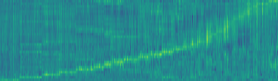
\includegraphics[interpolate=true,width=2.780000in,height=0.810000in]{figures/first_layer-img5.png}}%
\end{pgfscope}%
\begin{pgfscope}%
\pgfsetbuttcap%
\pgfsetroundjoin%
\definecolor{currentfill}{rgb}{0.000000,0.000000,0.000000}%
\pgfsetfillcolor{currentfill}%
\pgfsetlinewidth{0.803000pt}%
\definecolor{currentstroke}{rgb}{0.000000,0.000000,0.000000}%
\pgfsetstrokecolor{currentstroke}%
\pgfsetdash{}{0pt}%
\pgfsys@defobject{currentmarker}{\pgfqpoint{0.000000in}{-0.048611in}}{\pgfqpoint{0.000000in}{0.000000in}}{%
\pgfpathmoveto{\pgfqpoint{0.000000in}{0.000000in}}%
\pgfpathlineto{\pgfqpoint{0.000000in}{-0.048611in}}%
\pgfusepath{stroke,fill}%
}%
\begin{pgfscope}%
\pgfsys@transformshift{4.123858in}{0.413580in}%
\pgfsys@useobject{currentmarker}{}%
\end{pgfscope}%
\end{pgfscope}%
\begin{pgfscope}%
\definecolor{textcolor}{rgb}{0.000000,0.000000,0.000000}%
\pgfsetstrokecolor{textcolor}%
\pgfsetfillcolor{textcolor}%
\pgftext[x=4.123858in,y=0.316358in,,top]{\color{textcolor}\rmfamily\fontsize{10.000000}{12.000000}\selectfont \(\displaystyle {200}\)}%
\end{pgfscope}%
\begin{pgfscope}%
\pgfsetbuttcap%
\pgfsetroundjoin%
\definecolor{currentfill}{rgb}{0.000000,0.000000,0.000000}%
\pgfsetfillcolor{currentfill}%
\pgfsetlinewidth{0.803000pt}%
\definecolor{currentstroke}{rgb}{0.000000,0.000000,0.000000}%
\pgfsetstrokecolor{currentstroke}%
\pgfsetdash{}{0pt}%
\pgfsys@defobject{currentmarker}{\pgfqpoint{0.000000in}{-0.048611in}}{\pgfqpoint{0.000000in}{0.000000in}}{%
\pgfpathmoveto{\pgfqpoint{0.000000in}{0.000000in}}%
\pgfpathlineto{\pgfqpoint{0.000000in}{-0.048611in}}%
\pgfusepath{stroke,fill}%
}%
\begin{pgfscope}%
\pgfsys@transformshift{4.848259in}{0.413580in}%
\pgfsys@useobject{currentmarker}{}%
\end{pgfscope}%
\end{pgfscope}%
\begin{pgfscope}%
\definecolor{textcolor}{rgb}{0.000000,0.000000,0.000000}%
\pgfsetstrokecolor{textcolor}%
\pgfsetfillcolor{textcolor}%
\pgftext[x=4.848259in,y=0.316358in,,top]{\color{textcolor}\rmfamily\fontsize{10.000000}{12.000000}\selectfont \(\displaystyle {400}\)}%
\end{pgfscope}%
\begin{pgfscope}%
\pgfsetbuttcap%
\pgfsetroundjoin%
\definecolor{currentfill}{rgb}{0.000000,0.000000,0.000000}%
\pgfsetfillcolor{currentfill}%
\pgfsetlinewidth{0.803000pt}%
\definecolor{currentstroke}{rgb}{0.000000,0.000000,0.000000}%
\pgfsetstrokecolor{currentstroke}%
\pgfsetdash{}{0pt}%
\pgfsys@defobject{currentmarker}{\pgfqpoint{0.000000in}{-0.048611in}}{\pgfqpoint{0.000000in}{0.000000in}}{%
\pgfpathmoveto{\pgfqpoint{0.000000in}{0.000000in}}%
\pgfpathlineto{\pgfqpoint{0.000000in}{-0.048611in}}%
\pgfusepath{stroke,fill}%
}%
\begin{pgfscope}%
\pgfsys@transformshift{5.572660in}{0.413580in}%
\pgfsys@useobject{currentmarker}{}%
\end{pgfscope}%
\end{pgfscope}%
\begin{pgfscope}%
\definecolor{textcolor}{rgb}{0.000000,0.000000,0.000000}%
\pgfsetstrokecolor{textcolor}%
\pgfsetfillcolor{textcolor}%
\pgftext[x=5.572660in,y=0.316358in,,top]{\color{textcolor}\rmfamily\fontsize{10.000000}{12.000000}\selectfont \(\displaystyle {600}\)}%
\end{pgfscope}%
\begin{pgfscope}%
\definecolor{textcolor}{rgb}{0.000000,0.000000,0.000000}%
\pgfsetstrokecolor{textcolor}%
\pgfsetfillcolor{textcolor}%
\pgftext[x=4.792118in,y=0.137346in,,top]{\color{textcolor}\rmfamily\fontsize{10.000000}{12.000000}\selectfont Filter index}%
\end{pgfscope}%
\begin{pgfscope}%
\pgfsetbuttcap%
\pgfsetroundjoin%
\definecolor{currentfill}{rgb}{0.000000,0.000000,0.000000}%
\pgfsetfillcolor{currentfill}%
\pgfsetlinewidth{0.803000pt}%
\definecolor{currentstroke}{rgb}{0.000000,0.000000,0.000000}%
\pgfsetstrokecolor{currentstroke}%
\pgfsetdash{}{0pt}%
\pgfsys@defobject{currentmarker}{\pgfqpoint{-0.048611in}{0.000000in}}{\pgfqpoint{-0.000000in}{0.000000in}}{%
\pgfpathmoveto{\pgfqpoint{-0.000000in}{0.000000in}}%
\pgfpathlineto{\pgfqpoint{-0.048611in}{0.000000in}}%
\pgfusepath{stroke,fill}%
}%
\begin{pgfscope}%
\pgfsys@transformshift{3.403079in}{0.413580in}%
\pgfsys@useobject{currentmarker}{}%
\end{pgfscope}%
\end{pgfscope}%
\begin{pgfscope}%
\definecolor{textcolor}{rgb}{0.000000,0.000000,0.000000}%
\pgfsetstrokecolor{textcolor}%
\pgfsetfillcolor{textcolor}%
\pgftext[x=3.236412in, y=0.365355in, left, base]{\color{textcolor}\rmfamily\fontsize{10.000000}{12.000000}\selectfont \(\displaystyle {0}\)}%
\end{pgfscope}%
\begin{pgfscope}%
\pgfsetbuttcap%
\pgfsetroundjoin%
\definecolor{currentfill}{rgb}{0.000000,0.000000,0.000000}%
\pgfsetfillcolor{currentfill}%
\pgfsetlinewidth{0.803000pt}%
\definecolor{currentstroke}{rgb}{0.000000,0.000000,0.000000}%
\pgfsetstrokecolor{currentstroke}%
\pgfsetdash{}{0pt}%
\pgfsys@defobject{currentmarker}{\pgfqpoint{-0.048611in}{0.000000in}}{\pgfqpoint{-0.000000in}{0.000000in}}{%
\pgfpathmoveto{\pgfqpoint{-0.000000in}{0.000000in}}%
\pgfpathlineto{\pgfqpoint{-0.048611in}{0.000000in}}%
\pgfusepath{stroke,fill}%
}%
\begin{pgfscope}%
\pgfsys@transformshift{3.403079in}{0.816147in}%
\pgfsys@useobject{currentmarker}{}%
\end{pgfscope}%
\end{pgfscope}%
\begin{pgfscope}%
\definecolor{textcolor}{rgb}{0.000000,0.000000,0.000000}%
\pgfsetstrokecolor{textcolor}%
\pgfsetfillcolor{textcolor}%
\pgftext[x=3.236412in, y=0.767922in, left, base]{\color{textcolor}\rmfamily\fontsize{10.000000}{12.000000}\selectfont \(\displaystyle {4}\)}%
\end{pgfscope}%
\begin{pgfscope}%
\pgfsetbuttcap%
\pgfsetroundjoin%
\definecolor{currentfill}{rgb}{0.000000,0.000000,0.000000}%
\pgfsetfillcolor{currentfill}%
\pgfsetlinewidth{0.803000pt}%
\definecolor{currentstroke}{rgb}{0.000000,0.000000,0.000000}%
\pgfsetstrokecolor{currentstroke}%
\pgfsetdash{}{0pt}%
\pgfsys@defobject{currentmarker}{\pgfqpoint{-0.048611in}{0.000000in}}{\pgfqpoint{-0.000000in}{0.000000in}}{%
\pgfpathmoveto{\pgfqpoint{-0.000000in}{0.000000in}}%
\pgfpathlineto{\pgfqpoint{-0.048611in}{0.000000in}}%
\pgfusepath{stroke,fill}%
}%
\begin{pgfscope}%
\pgfsys@transformshift{3.403079in}{1.218714in}%
\pgfsys@useobject{currentmarker}{}%
\end{pgfscope}%
\end{pgfscope}%
\begin{pgfscope}%
\definecolor{textcolor}{rgb}{0.000000,0.000000,0.000000}%
\pgfsetstrokecolor{textcolor}%
\pgfsetfillcolor{textcolor}%
\pgftext[x=3.236412in, y=1.170489in, left, base]{\color{textcolor}\rmfamily\fontsize{10.000000}{12.000000}\selectfont \(\displaystyle {8}\)}%
\end{pgfscope}%
\begin{pgfscope}%
\pgfsetrectcap%
\pgfsetmiterjoin%
\pgfsetlinewidth{0.803000pt}%
\definecolor{currentstroke}{rgb}{0.000000,0.000000,0.000000}%
\pgfsetstrokecolor{currentstroke}%
\pgfsetdash{}{0pt}%
\pgfpathmoveto{\pgfqpoint{3.403079in}{0.413580in}}%
\pgfpathlineto{\pgfqpoint{3.403079in}{1.218714in}}%
\pgfusepath{stroke}%
\end{pgfscope}%
\begin{pgfscope}%
\pgfsetrectcap%
\pgfsetmiterjoin%
\pgfsetlinewidth{0.803000pt}%
\definecolor{currentstroke}{rgb}{0.000000,0.000000,0.000000}%
\pgfsetstrokecolor{currentstroke}%
\pgfsetdash{}{0pt}%
\pgfpathmoveto{\pgfqpoint{6.181157in}{0.413580in}}%
\pgfpathlineto{\pgfqpoint{6.181157in}{1.218714in}}%
\pgfusepath{stroke}%
\end{pgfscope}%
\begin{pgfscope}%
\pgfsetrectcap%
\pgfsetmiterjoin%
\pgfsetlinewidth{0.803000pt}%
\definecolor{currentstroke}{rgb}{0.000000,0.000000,0.000000}%
\pgfsetstrokecolor{currentstroke}%
\pgfsetdash{}{0pt}%
\pgfpathmoveto{\pgfqpoint{3.403079in}{0.413580in}}%
\pgfpathlineto{\pgfqpoint{6.181157in}{0.413580in}}%
\pgfusepath{stroke}%
\end{pgfscope}%
\begin{pgfscope}%
\pgfsetrectcap%
\pgfsetmiterjoin%
\pgfsetlinewidth{0.803000pt}%
\definecolor{currentstroke}{rgb}{0.000000,0.000000,0.000000}%
\pgfsetstrokecolor{currentstroke}%
\pgfsetdash{}{0pt}%
\pgfpathmoveto{\pgfqpoint{3.403079in}{1.218714in}}%
\pgfpathlineto{\pgfqpoint{6.181157in}{1.218714in}}%
\pgfusepath{stroke}%
\end{pgfscope}%
\begin{pgfscope}%
\definecolor{textcolor}{rgb}{0.000000,0.000000,0.000000}%
\pgfsetstrokecolor{textcolor}%
\pgfsetfillcolor{textcolor}%
\pgftext[x=4.792118in,y=1.302048in,,base]{\color{textcolor}\rmfamily\fontsize{12.000000}{14.400000}\selectfont (f) wav2vec 2.0 FE}%
\end{pgfscope}%
\end{pgfpicture}%
\makeatother%
\endgroup%


\subsubsection{Larger Supervised Convolutional Architecture}
\label{sec:scf_size}
As a larger inner dimension clearly showed better performance for the \wvtwo \gls{FE}, we increase the inner dimensions of the \gls{SC} features as well.
However, as shown in \refTab{table:features_scf_size}, neither increasing the number of filters operating on the waveform nor the number of kernels for the multi-resolutional temporal integration helps to improve the performance.
Note that the number of parameters of the full model is even larger than for the \wvtwo model in \refTab{table:features_general}, however, a large portion of those parameters is consumed by the linear projection of the features after the \gls{VGG} block.

\begin{table}[htbp]

\centering
\caption{Comparison of different inner dimensions for learnable \acrfull{SC} feature extraction.}
\label{table:features_scf_size}
\begin{tabular}{|c|c|c|c|S|}
\hline
 \#Waveform & \#Temp. Integr. & \multicolumn{2}{c|}{\#Params} & {WER} \\\cline{3-4}
Filterbanks &         Kernels &                         Total &  FE &       \\\hline
          5 &             100 &                         81.1M & 27k &   7.1 \\\cline{2-5}
            &             150 &                         85.2M & 40k &   7.1 \\\cline{2-5}
            &             200 &                         89.3M & 53k &   7.1 \\\cline{2-5}
            &             250 &                         93.4M & 67k &   7.3 \\\hline
          6 &             150 &                         87.7M & 40k &   7.3 \\\cline{1-1}\cline{3-5}
          7 &                 &                         90.1M & 41k &   7.1 \\
\hline
\end{tabular}

\end{table}


\subsubsection{First Layer Window Size}
\label{sec:scf_first_window}
Furthermore, the effect of the first layer's window size is studied and the results are shown in \refTab{table:features_window_size}.
They suggest that smaller window sizes than in \cite{tuske2018:waveform} perform better in the context of a \conformer \gls{CTC} model.
In particular, it does not seem to be necessary to cover one full pitch period which is around \ms{16} for low voices.
Instead, the best result is achieved with a window size of \ms{10} and even smaller windows still achieve comparable performance.
Note that all experiments in \refSec{sec:scf_size} use a window size of \ms{16}.

\begin{table}[htbp]

\centering
\caption{Comparison of different sizes for the layer which operates directly on the waveform in the learnable \acrfull{SC} feature extraction.}
\label{table:features_window_size}
\begin{tabular}{|c|c|S|c|S|c|}
\hline
\multicolumn{2}{|c|}{Window Size} & \multicolumn{4}{c|}{{WER [\%]}} \\\cline{3-6}
           \multicolumn{2}{|c|}{} &      \multicolumn{2}{c|}{{dev}} & \multicolumn{2}{c|}{{test}} \\\hline
                       in samples & in \si{\milli\second} &                         {clean} & other &                     {clean} & other \\\hline\hline
                               64 &                     4 &                             3.0 &   7.2 &                         3.4 &   7.8 \\\hline
                              128 &                     8 &                             3.0 &   7.1 &                         3.3 &   7.6 \\\hline
                              160 &                    10 &                             2.9 &   7.0 &                         3.4 &   7.6 \\\hline
                              256 &                    16 &                             3.0 &   7.1 &                         3.4 &   7.7 \\\hline
                              400 &                    25 &                             2.9 &   7.3 &                         3.4 &   7.7 \\
\hline
\end{tabular}

\end{table}


\subsection{\wvtwo Pre-Training}
The main appeal of the \wvtwo framework is the ability to pre-train the model on unlabeled audio data.
\cite{facebook2020wav2vec2} even reports relative \gls{WER} improvements of about 10\% on the \textit{other} subsets for their experiments on LibriSpeech when pre-training on the same data as used in supervised training compared to pure supervised training from scratch.
Here, we study this effect for the \fe only by using the parameters of an \fe pre-trained on LibriSpeech\footnote{\raggedright\url{https://github.com/facebookresearch/fairseq/blob/main/examples/wav2vec/README.md}}, so no external data is added.
During the supervised training, the \fe weights can be further trained or kept frozen.
As shown in \refTab{table:features_pretraining}, no positive effect can be observed here.
In fact, using a frozen pre-trained \fe shows clearly worse performance than training the \fe purely supervised from scratch.
We hypothesize that the pre-training mainly benefits the \transformer encoder and not the \fe while the mismatch between the \transformer encoder in pre-training and \conformer encoder in our setup could also pose a challenge for the case that the \fe is frozen.

\begin{table}[htbp]

\centering
\caption{Effect of pre-training the wav2vec 2.0 feature extractor using the unsupervised loss on the same data (Librispeech 960h).}
\label{table:features_pretraining}
\begin{tabular}{|c|c|S|}
\hline
\multicolumn{2}{|c|}{Feature Extractor} &       {WER} \\\hline
                              Trainable & Pretrained & {dev-other} \\\hline
                                    yes &         no &         6.8 \\\cline{2-3}
                                        &        yes &         6.9 \\\cline{1-1}\cline{3-3}
                                     no &            &         7.1 \\
\hline
\end{tabular}

\end{table}


\subsection{Frequency Response of Learned Filters}
Finally, we analyze the learned filters of the neural \fes.
First, the frequency response of the filters in the first layer which operates on the raw waveform is plotted.
As the order of learned filters in a convolutional layer is arbitrary, we sort the filters by the peak value of the frequency response and by the upper and lower \SI{3}{\decibel} cutoff frequencies as second and third criteria, respectively.
The plots are depicted in \refFig{fig:first_layer}\,(a)-(d), which share the same color range.

The well known distribution of the Gammatone filters is given in \refFig{fig:first_layer}\,(a) as a reference.
\refFig{fig:first_layer}\,(b) shows the frequency response of the learned \gls{SC} filters.
In line with \cite{tuske2018:waveform}, bandpass filters with a non-linear distribution of center frequencies are learned.
This confirms, that these filters are also preferred by more advanced neural back-ends like self-attention-based like \conformer which are superior in the exploitation of context information compared to simpler neural back-ends e.g. in \cite{tuske2014raw}.
The distribution resembles the Gammatone filterbank and with higher center frequencies, the pass band is also wider.
However, the stopband attenuation is clearly weaker and there is also a number of filters with no clear passband and a rather uncharacteristic frequency response.
This is particularly visible in \refFig{fig:first_layer}\,(e).

The distribution for the \wvtwo \fe's first layer in \refFig{fig:first_layer}\,(c) does not entail this degree of resemblance.
Again, bandpass filters are learned, however, they have a wider passband, their center frequencies are distributed rather linearly and the stopband attenuation is weak.
In addition, about 14\% of all filters have their peak at \SI{0}{\kilo\hertz} and another 10\% at \SI{8}{\kilo\hertz} with varying bandwidths.
Moreover, a number of filters exists with multiple passbands.
Interestingly, the frequency response of the pre-trained \wvtwo \fe in \refFig{fig:first_layer}\,(d) is very similar to \refFig{fig:first_layer}\,(c).
This indicates that the properties learned in unsupervised pre-training and supervised \gls{CTC} training are similar.

\section{Conclusions}

\section{Acknowledgements}

\ifinterspeechfinal
     The authors would like to thank Wei Zhou for providing the baseline \gls{CTC} model.
\else
     The acknowledgements would likely reveal the author identity and are therefore hidden for the double-blind review process.
\fi

{
\color{red}
\section{To Dos/Questions}
\begin{itemize}
  \item check for arxiv citations
\end{itemize}
}

\bibliographystyle{IEEEtran}
\bibliography{mybib}

\end{document}
